\documentclass[10pt,a4]{article}
%\documentclass[10pt,a4,twocolumn]{article}
%\documentclass[floatfix,showkeys,nopreprint]{jasatex}


\usepackage{amsmath,amsfonts,amssymb}% popular packages from the American Mathematical Society
\usepackage{bm}% Bold Math package
%\usepackage[]{color}
\usepackage[]{epsfig}
\usepackage[]{subfigure}
%\usepackage{fancyheadings} obsolete
\usepackage{fancyhdr}
%\usepackage[comma,square,sort&compress]{natbib}
\usepackage{ifthen}
\newboolean{TEX4HT}

%\usepackage[]{multicolumn}
%\usepackage[]{showlabels}

\setboolean{TEX4HT}{false}

\usepackage[colorlinks=true,linkcolor=blue,ps2pdf]{hyperref}
\title{\textbf{User Manual for the DREAM Toolbox\\
    Version \version}\\
  An ultrasound simulation software for use with
  \href{http://www.mathworks.com}{\textsc{Matlab}}
  and
  \href{http://www.octave.org}{\textsc{GNU Octave}}}

\author{Fredrik Lingvall\footnote{\texttt{https://github.com/frli8848/DREAM}}}

%\usepackage[colorlinks=true,linkcolor=blue,tex4ht]{hyperref}
%\newcommand{\url}[1]{(\ensuremath{\texttt{#1}})}
%\newcommand{\href}[2]{\ensuremath{(\texttt{#1})\texttt{#2}}}


\input{version.tex} % Get version info from CMake

\usepackage{xspace}
\setlength{\textheight}{220mm}
\setlength{\textwidth}{160mm}
\setlength{\oddsidemargin}{0mm}
\setlength{\evensidemargin}{0mm}
\setlength{\topmargin}{0mm}
\setlength{\headheight}{0mm}
\setlength{\headsep}{11mm}

\setlength{\parskip}{1.3mm}

\renewcommand{\subfigcapmargin}{0pt}
\renewcommand{\subfigtopskip}{5pt}
\renewcommand{\subfigcapskip}{0pt}
\renewcommand{\subfigbottomskip}{0pt}

% IEEE stuff
\newcommand{\IEEEuffc}{IEEE Transactions on Ultrasonics\mbox{,} Ferroelectrics\mbox{,} and Frequency Control}
\newcommand{\IEEEsu}{IEEE Transactions on Sonics and Ultrasonics}
\newcommand{\IEEEassp}{IEEE Transactions on Acoustics\mbox{,} Speech, and Signal Processing}
\newcommand{\IEEEbe}{IEEE Transactions on Biomedical Engeering}
\newcommand{\IEEEproc}{Proceedings of the IEEE}
\newcommand{\IEEEaes}{IEEE Transactions on Aerospace and Electronic Systems}
\newcommand{\IEEEoe}{IEEE Journal of Oceanic Engineering}
\newcommand{\IEEEmi}{IEEE Transactions on Medical Imaging}
\newcommand{\IEEEac}{IEEE Transactions on Automatic Control}
\newcommand{\IEEEit}{Transactions on Information Theory}
\newcommand{\IEEEus}{IEEE Ultrasonics Symposium}

%\renewcommand{\baselinestretch}{1.5}
%\AtBeginDelayedFloats{\renewcommand{\baselinestretch}{1.5}}


%\newcounter{tmpenumi}
\def\PARstart#1#2{\begingroup\def\par{\endgraf\endgroup\lineskiplimit=0pt}
  \setbox2=\hbox{\uppercase{#2} }\newdimen\tmpht \tmpht \ht2
  \advance\tmpht by \baselineskip\font\hhuge=cmr10 at \tmpht
  \setbox1=\hbox{{\hhuge #1}}
  \count7=\tmpht \count8=\ht1\divide\count8 by 1000 \divide\count7 by\count8
  \tmpht=.001\tmpht\multiply\tmpht by \count7\font\hhuge=cmr10 at \tmpht
  \setbox1=\hbox{{\hhuge #1}} \noindent \hangindent1.05\wd1
  \hangafter=-2 {\hskip-\hangindent \lower1\ht1\hbox{\raise1.0\ht2\copy1}%
    \kern-0\wd1}\copy2\lineskiplimit=-1000pt}

\lhead{\scalebox{0.2}{
\epsfig{file=userman/eps/dream_logo.eps}}} %Tar bort Section titeln fr�n toppen p� sidan.
\input{revision.tex} % \rhead def.
%\rhead{\fancyplain{}{Lingvall, \thepage}}

\usepackage{amsthm}
\newtheoremstyle{example}% name
{3pt}%      Space above
{3pt}%      Space below
{}%         Body font
{\parindent}%         Indent amount (empty = no indent, \parindent = para indent)
{\bfseries}% Thm head font
{.}%        Punctuation after thm head
{.5em}%     Space after thm head: " " = normal interword space;
% \newline = linebreak
{}%   Thm head spec (can be left empty, meaning `normal')

%\theoremstyle{plain}
%\theoremstyle{defintion}
%\theoremstyle{remark}
\theoremstyle{example}
%\newtheorem*{example}{Example} % unnumbered.
\newtheorem{example}{Example}
%\newtheorem{example}[theorem]{Example} Usig counter "theorem"

%
% Some useful definitions.
%

% Small math text (for capital subscripts in math).
\newcommand{\smt}[1]{\ensuremath{\textsc{#1}}}
% Math text (for subscripts in math).
\newcommand{\mt}[1]{\ensuremath{\text{#1}}}
% Bold symbol.
\newcommand{\bs}[1]{\ensuremath{\boldsymbol{#1}}}

%
% tex4ht do not like macros using "_\text{s}"
%

\ifthenelse{\boolean{TEX4HT}}
{
  \newcommand{\rs}{\ensuremath{\mathbf{r}_s}}
  \newcommand{\ro}{\ensuremath{\mathbf{r}_o}}
}{
  \newcommand{\rs}{\ensuremath{\mathbf{r}_{\text{s}}}}
  \newcommand{\ro}{\ensuremath{\mathbf{r}_{\text{o}}}}
}

\newcommand{\rr}{\ensuremath{\mathbf{r}}}
\newcommand{\rect}[1]{\ensuremath{\text{rect}(#1)}}


\newcommand{\Matlab}{\textsc{Matlab}}
\newcommand{\matlab}{\textsc{Matlab}}
\newcommand{\Octave}{\textsc{Octave}}
\newcommand{\octave}{\textsc{Octave}}

% The vec operator (vec is allready defined hence mvec).
\newcommand{\mvec}[1]{\ensuremath{\operatorname{vec}(#1)}\xspace}

\newcommand{\fourier}[1]{\ensuremath{\mathcal{F}\{#1\}}\xspace}
\newcommand{\ifourier}[1]{\ensuremath{\mathcal{F}^{-1}\{#1\}}\xspace}

\ifthenelse{\boolean{TEX4HT}}
{
  \newcommand{\cp}{\ensuremath{c_p}}
  \newcommand{\cs}{\ensuremath{c_s}}
  \newcommand{\ts}{\ensuremath{T_s}}
  \newcommand{\Ts}{\ensuremath{T_s}}
  \newcommand{\fs}{\ensuremath{F_s}}
  \newcommand{\Fs}{\ensuremath{F_s}}
}{
  \newcommand{\cp}{\ensuremath{c_\text{p}}}
  \newcommand{\cs}{\ensuremath{c_\text{s}}}
  \newcommand{\ts}{\ensuremath{T_\text{s}}}
  \newcommand{\Ts}{\ensuremath{T_\text{s}}}
  \newcommand{\fs}{\ensuremath{F_\text{s}}}
  \newcommand{\Fs}{\ensuremath{F_\text{s}}}
}


\newcommand{\R}{\ensuremath{\mathbf{R}}}

\newcommand{\A}{\ensuremath{\mathbf{A}}}
\renewcommand{\a}{\ensuremath{\mathbf{a}}}
\newcommand{\D}{\ensuremath{\mathbf{D}}}
\renewcommand{\d}{\ensuremath{\mathbf{d}}}

\renewcommand{\H}{\ensuremath{\mathbf{H}}}
\newcommand{\h}{\ensuremath{\mathbf{h}}}

% Can also use \eye in misc.sty
\newcommand{\I}{\ensuremath{\mathbf{I}}}

\renewcommand{\S}{\ensuremath{\mathbf{S}}}
\newcommand{\U}{\ensuremath{\mathbf{U}}}
\newcommand{\V}{\ensuremath{\mathbf{V}}}

\renewcommand{\u}{\ensuremath{\mathbf{u}}}

\renewcommand{\P}{\ensuremath{\mathbf{P}}}
\newcommand{\p}{\ensuremath{\mathbf{p}}}
\newcommand{\Pt}{\ensuremath{\mathbf{P}^T}}
\newcommand{\Y}{\ensuremath{\mathbf{Y}}}
\newcommand{\x}{\ensuremath{\mathbf{x}}}
\newcommand{\y}{\ensuremath{\mathbf{y}}}
\renewcommand{\o}{\ensuremath{\mathbf{o}}}
\renewcommand{\O}{\ensuremath{\mathbf{O}}}

\newcommand{\e}{\ensuremath{\mathbf{e}}}
\renewcommand{\r}{\ensuremath{\mathbf{r}}}

\newcommand{\n}{\ensuremath{\mathbf{n}}}
\newcommand{\se}{\ensuremath{s_\text{e}}}

%%\newcommand{\sf}{\ensuremath{S_\text{f}}}
%%\newcommand{\sb}{\ensuremath{S_\text{b}}}

\newcommand{\K}{\ensuremath{\mathbf{K}}}
\newcommand{\Kmmse}{\ensuremath{\mathbf{K}_\smt{mmse}}}
\newcommand{\Kopt}{\ensuremath{\mathbf{K}_\smt{opt}}}
\newcommand{\Klmmse}{\ensuremath{\mathbf{K}_\smt{lmmse}}}
\newcommand{\Kmap}{\ensuremath{\mathbf{K}_\smt{map}}}
\newcommand{\C}{\ensuremath{\mathbf{C}}}
\ifthenelse{\boolean{TEX4HT}}
{
  \newcommand{\Co}{\ensuremath{\mathbf{C}_{{o}}}}
  \newcommand{\Ce}{\ensuremath{\mathbf{C}_{{e}}}}
  \newcommand{\Coinv}{\ensuremath{{\mathbf{C}_o}^{-1}}}
  \newcommand{\Ceinv}{\ensuremath{{\mathbf{C}_e}^{-1}}}
  \newcommand{\Cerr}{\ensuremath{\mathbf{C}_\epsilon}}
  \newcommand{\cerr}{\ensuremath{\sigma_\epsilon}^2}
  \newcommand{\Eerr}{\ensuremath{\mathbf{E}_\epsilon}}
  \newcommand{\sigmae}{\ensuremath{\sigma_{{e}}^2}}
  \newcommand{\sigmao}{\ensuremath{\sigma_{{o}}^2}}
  \newcommand{\lambdao}{\ensuremath{\lambda_{{o}}}}
}{
  \newcommand{\Co}{\ensuremath{\mathbf{C}_{\text{o}}}}
  \newcommand{\Ce}{\ensuremath{\mathbf{C}_{\text{e}}}}
  \newcommand{\Coinv}{\ensuremath{\mathbf{C}_\text{o}^{-1}}}
  \newcommand{\Ceinv}{\ensuremath{\mathbf{C}_\text{e}^{-1}}}
  \newcommand{\Cerr}{\ensuremath{\mathbf{C}_\epsilon}}
  \newcommand{\cerr}{\ensuremath{\sigma_\epsilon}^2}
  \newcommand{\Eerr}{\ensuremath{\mathbf{E}_\epsilon}}
  \newcommand{\sigmae}{\ensuremath{\sigma_{\text{e}}^2}}
  \newcommand{\sigmao}{\ensuremath{\sigma_{\text{o}}^2}}
  \newcommand{\lambdao}{\ensuremath{\lambda_{\text{o}}}}
}

% Trace
\newcommand{\tr}[1]{\ensuremath{\operatorname{tr}\{#1\}}\xspace}

% Diagonal operator. (allready defined)
\newcommand{\diag}[1]{\ensuremath{\operatorname{diag}\{#1\}}\xspace}

% Expectation
\newcommand{\E}[1]{\ensuremath{\operatorname{E}\{#1\}}\xspace}

%\date{}

\begin{document}

\maketitle

%\vspace{1cm}
%\begin{center}
  %\mbox{\scalebox{0.8}{\mbox{\epsfig{file=userman/eps/frontpage.eps}}}}
  %\mbox{\scalebox{1.0}{\mbox{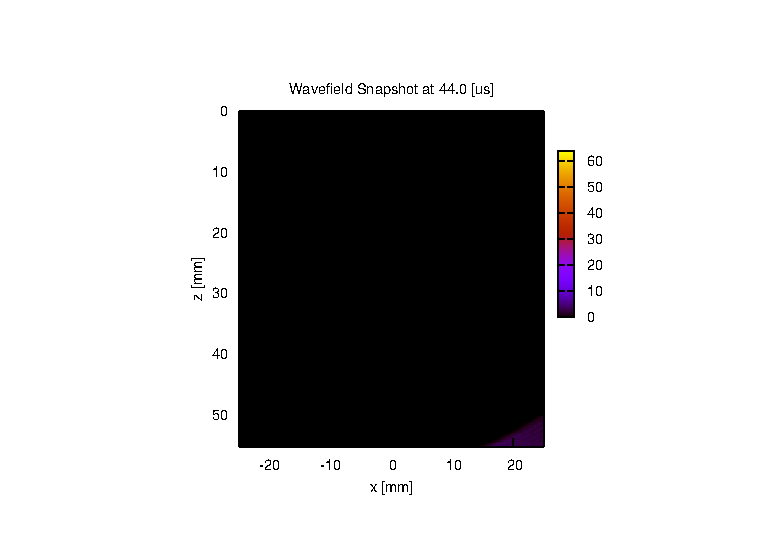
\epsfig{file=userman/eps/snapshot_50_m20.eps}}}}
  %\mbox{\epsfig{file=userman/eps/imp_resp.eps,width=0.38\columnwidth}
  %  \epsfig{file=userman/eps/freq_imp_resp.eps,width=0.38\columnwidth}}\\
  %\mbox{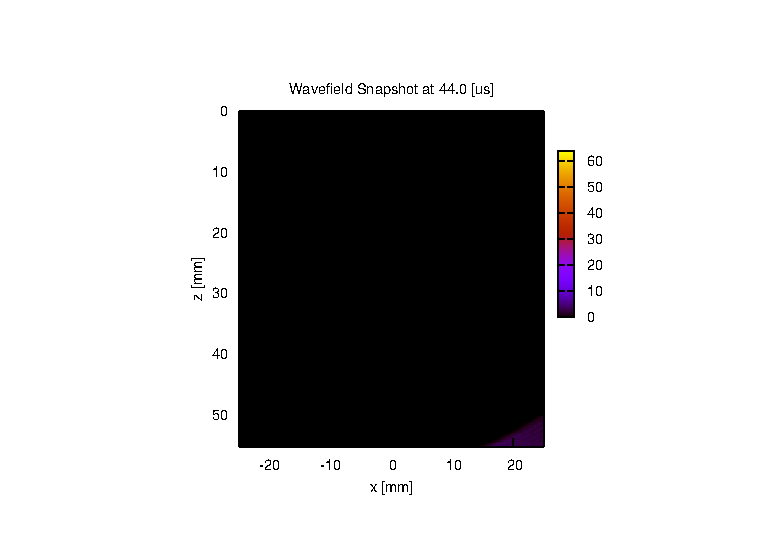
\epsfig{file=userman/eps/snapshot_50_m20.eps,width=0.68\columnwidth}}
  %
  %\mbox{\epsfig{file=userman/eps/snapshot_50_m20_4.0.eps,width=0.4\columnwidth}
  %  \epsfig{file=userman/eps/snapshot_50_m20_8.0.eps,width=0.4\columnwidth}}\\
  %\mbox{\epsfig{file=userman/eps/snapshot_50_m20_16.0.eps,width=0.4\columnwidth}
  %  \epsfig{file=userman/eps/snapshot_50_m20_24.0.eps,width=0.4\columnwidth}}\\
  %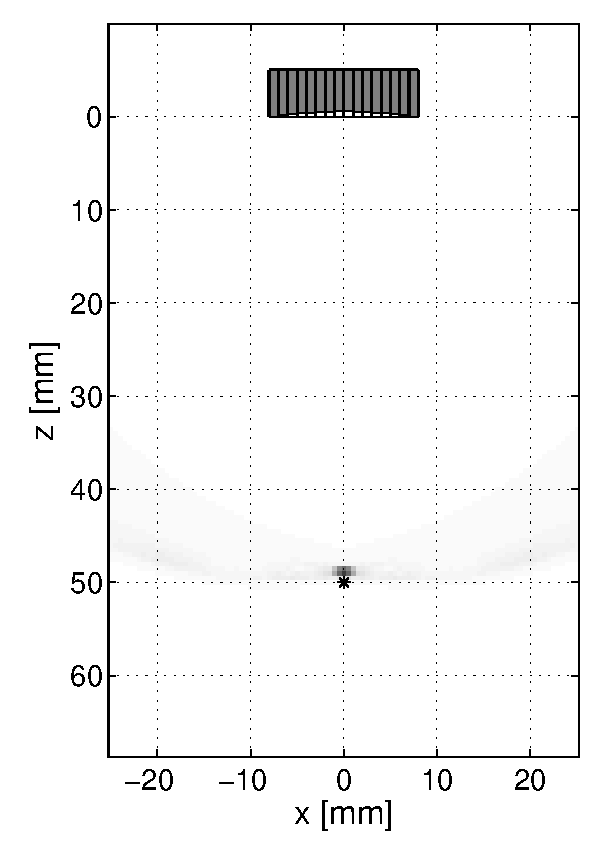
\epsfig{file=userman/eps/snapshot_foc_16_0280_bw.eps,width=0.4\columnwidth}
%\end{center}

%\newpage

%\begin{abstract}
%Nothing here yet...
%\end{abstract}

\newpage

\tableofcontents

\newpage

\pagestyle{fancy}

%\twocolumn

\section{Introduction}
\label{sec:intro}

\PARstart{T}{he} DREAM (Discrete REpresentation Array Modeling) toolbox is an open source software,
released under the GNU General Public License (GPL), for both \Matlab\ and Octave for simulating acoustic
fields radiated from common ultrasonic transducer types and arbitrarily complicated ultrasonic transducers
arrays. The DREAM toolbox enables analysis of beam steering, beam focusing, and apodization
for wide band (pulse) excitation both in near and far fields. The toolbox is also
provided with a user friendly graphical user interface (GUI).

The toolbox consists of a set of routines for computing (discrete) spatial impulse
response (SIRs) for various single-element transducer geometries as well as multi-element
transducer arrays. Based on linear systems theory, these SIR functions can then be
convolved with the transducer's electrical impulse response to obtain the acoustic field
at an observation point. %~\cite{Lhemery1991}.
Using the DREAM toolbox one can simulate ultrasonic measurement
systems for many configurations including phased arrays and measurements performed in
lossy media.

The DREAM toolbox uses a numerical procedure based on based on the discrete
representation (DR) computational concept~\cite{Piwakowski1989,Piwakowski1999} which is a method
based on the general approach of the spatial impulse responses~\cite{Tupholme1969,Stepanishen1971a}.

%\subsection{Outline of the Toolbox}
%
%The DREAM toolbox consists of set of \emph{user functions} that is called by the user
%from \Matlab/Octave (or from a script/function) and a set of \emph{helper
%functions} that is used internally in the DREAM toolbox. The DREAM toolbox also comes
%with a GUI (for \Matlab\ only) from which one call the different transducer functions
%and plot the SIRs for various configurations.

\section{Copyright}

\PARstart{T}{he} DREAM toolbox is an open source software and the source code for the toolbox is freely
redistributable under the terms of the GNU General Public License (GPL)
as published by the Free Software Foundation (\url{http://www.gnu.org}).
See also the file \texttt{COPYING} which is distributed with the DREAM Toolbox.

% TODO: update the webpage at http://www.signal.uu.se with current info
%
% The DREAM Toolbox can be downloaded at:
% %
% \url{http://www.signal.uu.se/Toolbox/dream/}.
% %
% At this website you can also find information how to contact the authors and report
% bugs etc.

\subsection{Disclaimer}

%\PARstart{T}{he}
The DREAM toolbox is distributed in the hope that it will
be useful but WITHOUT ANY WARRANTY. More specifically:
\begin{quote}
  \footnotesize
  THE PROGRAM IS PROVIDED ``AS-IS'' WITHOUT WARRANTY OF ANY KIND, EITHER EXPRESS OR IMPLIED, INCLUDING
  BUT NOT LIMITED TO THE IMPLIED WARRANTIES OR CONDITIONS OF MERCHANTABILITY OR FITNESS FOR A PARTICULAR
  PURPOSE. IN NO EVENT SHALL ANY OF THE AUTHORS OF THE DREAM TOOLBOX AND/OR THE DEPARTMENT OF ENGINEERING
  SCIENCES AT UPPSALA UNIVERSITY, SWEDEN, OR THE INSTITUT D'ELECTRONIQUE ET DE MICRU\--ELEC\-TRONIQUE DU NORD
  (IEMN-DOAE-UMR CNRS 9929), ECOLE CENTRALE DE LILLE, FRANCE, BE LIABLE FOR ANY SPECIAL, INCIDENTAL, INDIRECT,
  OR CONSEQUENTIAL DAMAGES OF ANY KIND, OR DAMAGES WHATSOEVER RESULTING FROM LOSS OF USE, DATA, OR PROFITS,
  WHETHER OR NOT THE AUTHORS OF THE DREAM TOOLBOX HAVE BEEN ADVISED OF THE POSSIBILITY OF SUCH DAMAGES,
  AND/OR ON ANY THEORY OF LIABILITY ARISING OUT OF OR IN CONNECTION WITH THE USE OR PERFORMANCE OF THIS
  SOFTWARE.
\end{quote}

% TODO
% \section{System Requirements}

% \begin{enumerate}

% \item \Matlab\ $\ge$ 7.1  or,

% \item \href{http://www.octave.org}{Octave} $\ge$ 3.8 recommended.

% \item \href{http://www.fftw.org}{FFTW} $\ge$ 3.0.1 (optional).\footnote{The attenuation code in DREAM makes heavily
%     use of FFTs. If the optimized \href{http://www.fftw.org}{FFTW} is installed then DREAM can be configured to use
%     this lib.} %Also, the \texttt{fftconv\_p} and \texttt{sum\_fftconv} functions needs the FFTW3 library.}

% \item Pthread.\footnote{If you want to use the parallel (threaded) DREAM functions in Windows you need to install
%   the Pthreads-Win32 library.}

% \end{enumerate}

\section{Installation}

\PARstart{T}{he} DREAM Toolbox can be installed both using pre-compiled binaries and from source code. Binaries are
currently available for Linux (x86\_64), Windows (x86\_64), and for macOS (Intel Macs). The binaries are compiled
using generic compiler flags and should, therefore, run on most setups.
%
If you want higher performance then it is recommended that you compile DREAM from source.

For more information see: \url{https://github.com/frli8848/DREAM#installation}

% TODO:
% \subsection{Octave Specific Installation Notes}
% \label{sec:oct-install}

% As mentioned above, the DREAM Toolbox must be installed from sources for Octave. Recent versions of
% Octave have a package manager tool (\texttt{pkg}) for that purpose. Given that you have the developer tools
% for your system installed (for Windows see Sections~\ref{sec:win_octave_mingw}) you should be able to
% install DREAM by,
% \begin{enumerate}

% \item Download the special DREAM source code file for the Octave package manager,

% \item type: \texttt{pkg install dream-{\version}.tar.gz} at the Octave command
%   line.\footnote{Note: this will not build the documentation.}

% \end{enumerate}
% %
% You should now be able to see the DREAM packege by typing:
% \begin{verbatim}
%   pkg list
% \end{verbatim}
% %
% at the Octave command line.


\section{An  Introduction to The Impulse Response Method}

\PARstart{T}{he} impulse response method is an approach based on linear systems theory to model acoustic fields from
ultrasonic transducers; the method was introduced by Tupholme and Stepanishen in the late 60's, early
70's~\cite{Tupholme1969,Stepanishen1971a}. The impulse response method is based on linear acoustics and can be used to
model acoustic fields and (double-path) responses for both single transducer setups and for array imaging. The idea
is to divide the imaging system in two parts: the first one accounts for acoustical wave propagation effects
(i.e., the diffraction effects) from the transducer surface to the observation point, and the second one accounts for
the electro-acoustical effects. These two parts are then convolved to obtain a model for the total imaging system.

The impulse response method is very flexible since, (\emph{i}) by linearity the response from multi-element transducers
(such as array transducers) can be obtained be means of super-position and (\emph{ii}) arbitrary input signals can be
treated by simply convolving the electro-acoustical impulse response with the input signal. In this section we will
present a short introduction to the impulse response method and, in particular, discuss how to use the method
for discrete-time modeling.

\subsection{The Baffled Piston Model and the Rayleigh Integral}
\label{sec:analythical}

The impulse response method is based on the assumption that the transducer can be treated as a
baffled piston. This assumption implies that we only need to consider the active area of the
transducer when modeling the wave propagation. That is, if the source (the transducer) is located
in the rigid plane, often referred to as the \emph{rigid baffle} as illustrated in
Figure~\ref{fig:integration}, then the baffle ($S_{\smt{b}}$) will not contribute to the field.
%%
\begin{figure}
  \begin{center}
    \scalebox{.5}{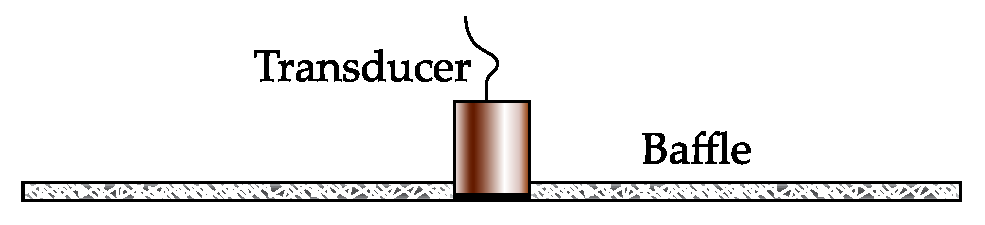
\epsfig{file=userman/eps/baffle.eps}}
  \end{center}
  \caption{Illustration of a baffled transducer.
    \label{fig:integration}}
\end{figure}
%
The pressure at an observation point $\rr$ is then described by the Rayleigh integral
%
\ifthenelse{\boolean{TEX4HT}}
{
  \begin{equation}
    \begin{split}
      p(\rr,t)  = &\rho_0 \frac{\partial}{\partial t} \int_{-\infty}^{\infty}
      \biggl( \int_{S_{\smt{r}}}  v_{{n}}(\rr_0, t_0) \frac{\delta\left(t - t_0 - |\rr - \rr_0|/c_p\right)}{2\pi |\rr -
        \mathbf{r}_0| }dS_{\smt{r}} \biggl) dt_0, \\
      = & \rho_0 \frac{\partial}{\partial t} \int_{-\infty}^{\infty}  v_{{n}}(t_0)
      \int_{S_{\smt{r}}} \frac{\delta\left(t - t_0 - |\rr - \rr_0|/c_p\right)}{2\pi |\rr - \mathbf{r}_0| }dS_{\smt{r}} dt_0, \\
      = & \rho_0 \frac{\partial}{\partial t} \int_{-\infty}^{\infty} v_{{n}}(t_0) h^{{f-}\smt{sir}}(\rr,t-t_0) dt_0, \\
      = & \rho_0 \frac{\partial}{\partial t} v_{{n}}(t) * h^{{f-}\smt{sir}}(\rr,t-t_0).
      \label{eq:rayleigh}
    \end{split}
  \end{equation}
}{
  \begin{equation}
    \begin{split}
      p(\rr,t)  = &\rho_0 \frac{\partial}{\partial t} \int_{-\infty}^{\infty}
      \biggl( \int_{S_{\smt{r}}}  v_{\text{n}}(\rr_0, t_0) \frac{\delta\left(t - t_0 - |\rr - \rr_0|/c_p\right)}{2\pi |\rr -
        \mathbf{r}_0| }dS_{\smt{r}} \biggl) dt_0, \\
      = & \rho_0 \frac{\partial}{\partial t} \int_{-\infty}^{\infty}  v_{\text{n}}(t_0)
      \int_{S_{\smt{r}}} \frac{\delta\left(t - t_0 - |\rr - \rr_0|/c_p\right)}{2\pi |\rr - \mathbf{r}_0| }dS_{\smt{r}} dt_0, \\
      = & \rho_0 \frac{\partial}{\partial t} \int_{-\infty}^{\infty} v_{\text{n}}(t_0) h^{\text{f-}\smt{sir}}(\rr,t-t_0) dt_0, \\
      = & \rho_0 \frac{\partial}{\partial t} v_{\text{n}}(t) * h^{\text{f-}\smt{sir}}(\rr,t-t_0).
      \label{eq:rayleigh}
    \end{split}
  \end{equation}
}
%
where it is where we for simplicity have assumed that the normal velocity
\ifthenelse{\boolean{TEX4HT}}
{
  $v_{{n}}(\rr_0, t) \equiv v_{{n}}(t)$ is
}{
  $v_{\text{n}}(\rr_0, t) \equiv v_{\text{n}}(t)$ is
}
uniform on the transducer's surface $S_{\smt{r}}$. The Rayleigh integral formula~\eqref{eq:rayleigh} simply states
that the acoustic field at an observation point is the sum of the contributions from all points of the active area
of the transducer. The impulse response
\ifthenelse{\boolean{TEX4HT}}
{
  $h^{{f-}\smt{sir}}(\rr,t)$
}{
  $h^{\text{f-}\smt{sir}}(\rr,t)$
}
in Eq.~\eqref{eq:rayleigh} is usually referred to
as the (forward) \emph{spatial impulse response} (SIR).

The normal velocity,
\ifthenelse{\boolean{TEX4HT}}
{
  $v_{{n}}(t)$,
}{
  $v_{\text{n}}(t)$,
}
depends on both the input signal, $u(t)$, and the electro-acoustical properties of the transducer, which can be
described with the (forward) electrical impulse response
\ifthenelse{\boolean{TEX4HT}}
{
  $h^{{ef}}(t)$.
}{
  $h^{\text{ef}}(t)$.
}
Thus, the pressure at $\rr$ can be expressed by the convolutions of the input signal and the two (forward)
impulse responses according to,
%
\ifthenelse{\boolean{TEX4HT}}
{
  \begin{equation}
    p(\rr,t) = h^{{f-}\smt{sir}}(\rr,t) * h^{{ef}}(t) * u(t).
    \label{eq:pressure_response}
  \end{equation}
}{
  \begin{equation}
    p(\rr,t) = h^{\text{f-}\smt{sir}}(\rr,t) * h^{\text{ef}}(t) * u(t).
    \label{eq:pressure_response}
  \end{equation}
}
%
Double-path (pulse-echo) responses can be treated in a similar way by convolving the forward
response~\eqref{eq:pressure_response} with the backward electrical (acousto-electrical) response
and the backward SIR for a point source at $\rr$.

Analytical solutions to SIRs exist for a few geometries, but one must in general
resort to numerical methods.
%%
Also, these \emph{time continuous} solutions are normally not practical since all acquired signals (the data) are
normally sampled and time discrete  models are, therefore, needed;
sampling of time continous SIRs is discussed in Section~\ref{sec:sir-sampling}.
%%
%In summary, the total system response can be modeled by convolving the electrical impulse response(s) and the
%SIRs.

Before we discuss sampled SIRs, and the particular method use by the DREAM Toolbox, let us consider a case where
there exist an analytical solution.
%
\begin{example}[The SIR for a Circular Disc]
  %
  The SIR of a circular disc (see illustration in Figure~\ref{fig:circ}) has an analytical
  solution~\cite{Stepanishen1971a}
  %%
  \begin{figure}[phtb]
    \begin{center}
      \scalebox{0.7}{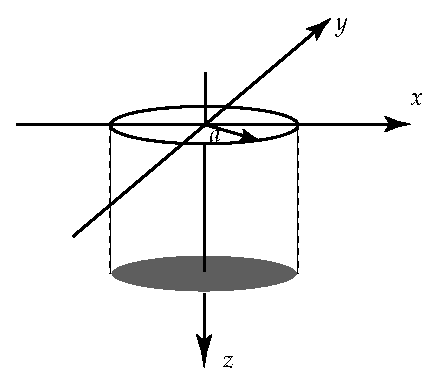
\epsfig{file=userman/eps/circ_aperture.eps}}
    \end{center}
    \caption{Geometry of a a circular disc source.
      \label{fig:circ}}
  \end{figure}
  %%
  which can be divided in two cases: (\emph{i})
  when the observation point is inside the aperture of the disc
  $\sqrt{x^2 + y^2}\le a$, where $a$ is the transducer radius, and (\emph{ii}) when the
  observation point is outside the aperture.
  The disc is assumed to be located in the $x$--$y$ plane centered at $x=y=0$. If we let $r$
  denote the distance in  the $x$--$y$ plane from the center axis of the disc to the observation point,
  $r  = \sqrt{x^2 + y^2}$, then the circular disc SIR is given by
  %%
  \ifthenelse{\boolean{TEX4HT}}
  {
    \begin{equation}
      \begin{split}
        {for}\ r \le a & \\
        h(\rr,t) & =
        \begin{cases}
          0, & \ \ t \le t_z \\
          \cp, &\ \ t_z \le t \le t_1 \\
          \frac{\cp}{\pi} \cos^{-1}\left(\cp^2 \frac{ t^2-t_z^2+t_r^2 - a/\cp^2}{2t_r\sqrt{t^2-t_z^2}}
          \right),\ &\ \ t_1 < t \le t_2 \\
          0, &\ \ t > t_2
        \end{cases} \\
        {for}\ r > a & \\
        h(\rr,t) & =
        \begin{cases}
          0, &\ \ t \le t_1 \\
          \frac{\cp}{\pi} \cos^{-1}\left(\cp^2\frac{t^2-t_z^2+t_r^2-a/\cp^2}{2t_r\sqrt{t^2-t_z^2}}
          \right),\ &\ \ t_1 <  t \le t_2 \\
          0, &\ \ t > t_2
        \end{cases} \\
      \end{split}
      \label{eq:disc}
    \end{equation}
  }{
    \begin{equation}
      \begin{split}
        \text{for}\ r \le a & \\
        h(\rr,t) & =
        \begin{cases}
          0, & \ \ t \le t_z \\
          \cp, &\ \ t_z \le t \le t_1 \\
          \frac{\cp}{\pi} \cos^{-1}\left(\cp^2 \frac{ t^2-t_z^2+t_r^2 - a/\cp^2}{2t_r\sqrt{t^2-t_z^2}}
          \right),\ &\ \ t_1 < t \le t_2 \\
          0, &\ \ t > t_2
        \end{cases} \\
        \text{for}\ r > a & \\
        h(\rr,t) & =
        \begin{cases}
          0, &\ \ t \le t_1 \\
          \frac{\cp}{\pi} \cos^{-1}\left(\cp^2\frac{t^2-t_z^2+t_r^2-a/\cp^2}{2t_r\sqrt{t^2-t_z^2}}
          \right),\ &\ \ t_1 <  t \le t_2 \\
          0, &\ \ t > t_2
        \end{cases} \\
      \end{split}
      \label{eq:disc}
    \end{equation}
  }
  %%
  where $t_z = z/\cp$ is the earliest time that the wave reaches the observation point
  $\rr$ when $r \le a$, $t_r = r/\cp$, and
  $t_{1,2} = t_z \sqrt{1 + (\frac{a\mp r}{z})^2}$
  are the propagation times corresponding to the edges of the disc that are
  closest and furthermost away from $\rr$, respectively.

  Noticeable is that the pulse amplitude of the on-axis SIR is constant
  regardless of the distance to the observation point.\footnote{The on-axis SIR
    has duration $t_1 - t_z$ with the constant amplitude $\cp$ in the time interval
    $t_z \le t \le t_1$.} The  duration of the on-axis SIR is given by
  $t_1=a/\cp$ at $z=0$. As the distance increases the duration, $t_1-t_z$, of the SIR
  becomes shorter, and for large $z$ it approaches to the delta function.
  %% the response of a point source.
  The transducer size effects are therefore most pronounced in the near-field.
  This is illustrated in Figure~\ref{fig:on_axis_sirs} where the on-axis SIRs at $z=20$ and
  $z=80$ mm, respectively are shown.
  %%
  \begin{figure}[phtb]
    \begin{center}
      \mbox{\subfigure[Spatial impulse response at $z=20$ mm.
        ]{\scalebox{0.4}{\epsfig{file=userman/eps/on_axis_close.eps}}}%\quad
        \subfigure[Spatial impulse response at $z=80$ mm.
        ]{\scalebox{0.4}{\mbox{\epsfig{file=userman/eps/on_axis_far.eps}}}}}
    \end{center}
    \caption{On-axis spatial impulse responses for a 10 mm disc where the sound
      speed, $\cp$, was 1500 m/s.
      \label{fig:on_axis_sirs}}
  \end{figure}
  %%
  The duration at $z=20$ is longer than that of $z=80$
  and if the distance, $z$, increases then the on-axis SIR will approach to a delta
  function, cf. Figures~\ref{fig:on_axis_sirs}(a) and (b).
  $\Box$
  \label{ex:circle}
\end{example}

As mentioned above, there exist no analytical analytical solutions for many transducer
geometries, and in such situations numerical methods must be used. The DREAM Toolbox uses a
method based on the \emph{discrete representation} (DR) computational concept~\cite{Piwakowski1989,Piwakowski1999}.
The DR method is very flexible in the sense that complex transducer shapes as well as arbitrary focusing
methods easily can be modeled. Another benefit of the DR method is that the SIRs are directly  computed in
a discrete form which is convenient since this directly allows for digital signal processing. The DR method
is described in Section~\ref{sec:dr} below, but first we will discuss sampling of spatial impulse responses.

\subsection{Discrete-time Spatial Impulse Responses}
\label{sec:sir-sampling}

Before we introduce the discrete representation (DR) method, which the DREAM toolbox transducer functions are
based on, let us discuss sampling of spatial impulse responses. This is of interest since our ultimate goal
normally is to model the total \emph{sampled} imaging system which includes both acoustic propagation effects (the SIRs)
as well as input signals and electro-acoustical effects.

To obtain a discrete model we need a discrete representation of the SIRs. That is, the analytical expressions
for the SIRs discussed in Section~\ref{sec:analythical} must be converted to a discrete form in order to be
useful for digital signal processing; a proper discrete representation of the SIRs
is necessary so that when the sampled SIR is convolved with the normal velocity the
resulting waveform can faithfully represent the sampled measured waveform.

The analytical SIRs have an infinite bandwidth due to the abrupt amplitude changes
that, for example, could be seen in the line and disc solutions above. In some
situations the duration of a SIR may even be shorter than the sampling interval,
$\ts$, and it is therefore not sufficient to simply sample the analytical SIRs by simply
taking the amplitude at the sampling instants %, $t_k$, %% for $k=0,1,\ldots,K-1$,
since the SIR may actually be zero those time instants.
%%
The SIRs are however convolved with a band-limited normal velocity signal, hence
the resulting pressure waveform must also be band-limited,
cf.~\eqref{eq:pressure_response}. Consequently, we only need to
sample the SIR in such way that the band-limited received A-scans
are properly modeled.

In a sampled system the impulse responses are given at discrete time instants, $t_k$ (given by the sampling
period $\Ts$) and to faithfully represent the SIRs we need to collect all contributions from the
continuous time SIRs in the corresponding sampling interval $[t_k-\Ts/2,t_k+\Ts/2]$.
%%
A discrete version of the a time continuous SIR is then obtained by summing all
contributions from the SIR in the actual sampling interval. That is, the
sampled SIR is defined as
%%
\begin{equation}
     h(\rr,t_k) \triangleq \frac{1}{\ts}
     \int_{t_k-\ts/2}^{t_k+\ts/2} h(\rr,t) dt.
\label{eq:sampled_sir}
\end{equation}
%%
The division by $\ts$ retains the same unit (m/s) of the sampled SIR as the continuous one.
The amplitude of the sampled SIR, at time $t_k$, is then the mean value of the
continuous SIR in the corresponding sampling interval, $[t_k-\ts/2, t_k+\ts/2]$.
%%
Also, as seen from the analytical solutions above, the SIRs always have a finite length
as the transducer has a finite size. The sampled SIRs are therefore naturally represented
by finite impulse response filters (FIRs).

The effect of the sampling scheme~\eqref{eq:sampled_sir} is illustrated in
Figure~\ref{fig:sampled_vs_analytic} for two discs with radii 1.2 and
3 mm, respectively, where the sampling interval, $\ts$, was 0.04$\mu$s.
%%
\begin{figure}[phtb]
  \begin{center}
    \subfigure[Continuous and sampled spatial impulse responses
    of a circular disc with radius $r=1.2$ mm.
    ]{\scalebox{0.4}{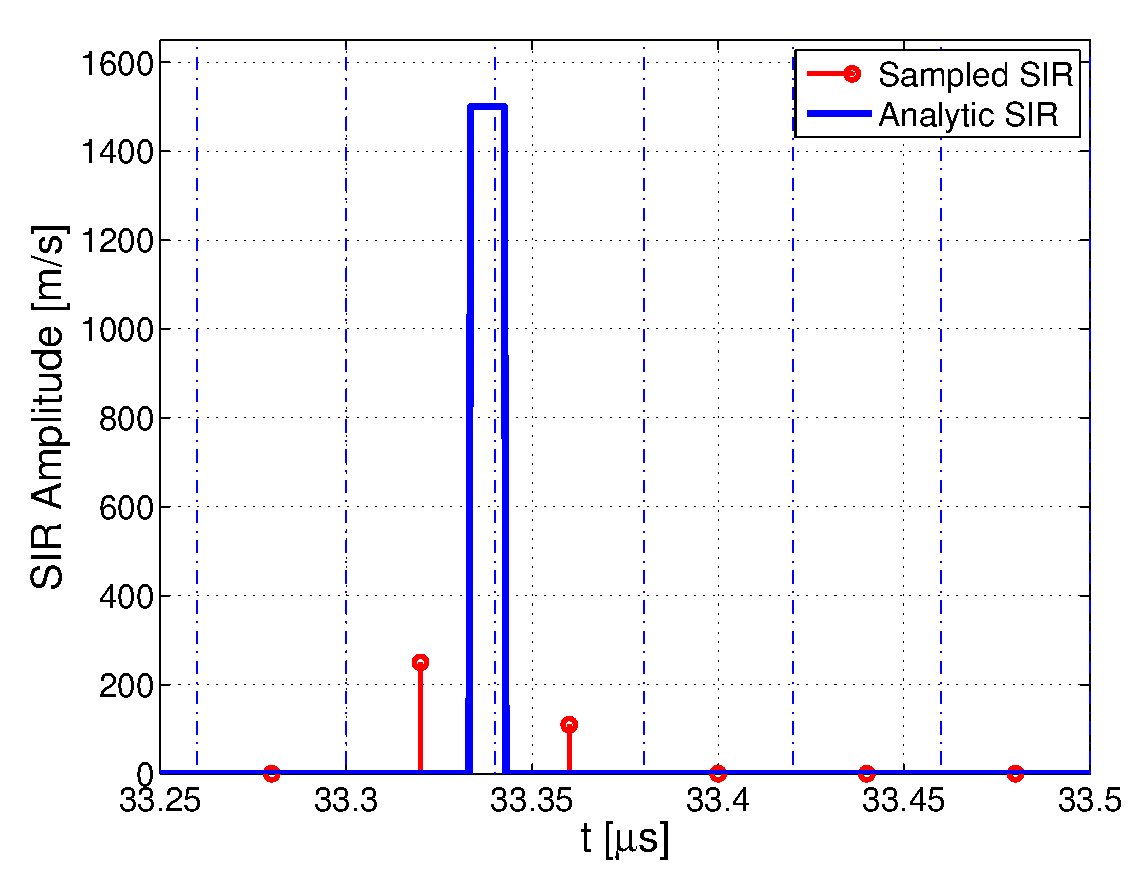
\epsfig{file=userman/eps/circ_sir_sampled_vs_analythic_small.eps}}}\quad
    \subfigure[Continuous and sampled spatial impulse responses
    of a circular disc with radius $r=3$ mm.
    ]{\scalebox{0.4}{\epsfig{file=userman/eps/circ_sir_sampled_vs_analythic_large.eps}}}
  \end{center}
  \caption{Illustration of sampling spatial impulse responses.
    The continuous and sampled on-axis SIRs for two discs with radii 1.2 and
    3 mm, respectively are shown where the sampling interval, $\ts$, was 0.04 $\mu$s
    (\cp = 1500 [m/s]).
    \label{fig:sampled_vs_analytic}}
\end{figure}
%%
In Figure~\ref{fig:sampled_vs_analytic}(a) the analytic SIR is shorter than the
sampling interval, $\ts$. The max amplitude of the discrete SIR is therefore lower
than then the max amplitude of the continuous SIR. If the duration of the analytic SIR
is longer than the sampling interval, as for the 3 mm disc shown in
Figure~\ref{fig:sampled_vs_analytic}(b), then the max amplitudes of the
on-axis sampled and analytic disc SIRs will be the same.

\subsection{The Discrete Representation (DR) Computational Concept}
\label{sec:dr}

As mentioned in previous in Section~\ref{sec:analythical}
the analytical spatial impulse responses are only available for a few simple
transducer geometries. Therefore, for a transducer with an arbitrary geometry a
numerical method must be used. The numerical method used in this toolbox is based on
the \emph{discrete representation} (DR) method, which is based on a discretization of the
Rayleigh integral formula~\eqref{eq:rayleigh}.
In the DR method, the radiating surface is divided into a set of
small surface elements (see illustration in Figure~\ref{fig:dream}), and
%%
\begin{figure}[phtb]
  \begin{center}
    \scalebox{0.6}{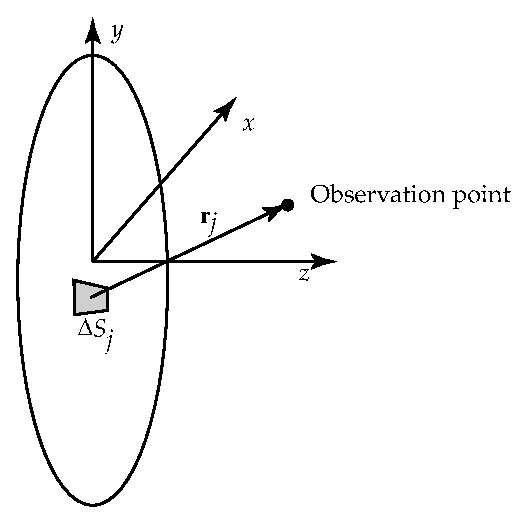
\epsfig{file=userman/eps/dream2.eps}}
  \end{center}
  \caption{Geometry and notations for the discrete representation method.
    \label{fig:dream}}
\end{figure}
%%
the surface integral in the Rayleigh formula is replaced by a summation.
The DR method facilitates computation
of SIRs for non-uniform excitation, apodization of the aperture, and arbitrary
focusing laws since each surface element can be assigned a different normal velocity,
apdodization or time-delay. The DR computational concept can therefore
be used for computing SIRs for an arbitrary transducer shape or array
layout~\cite{Piwakowski1999,Piwakowski1989}.

A discrete SIR, computed using the DR method, can be found by first dividing the total transducer surface
into a set of $J$ surface elements $\{\Delta S_0, \Delta S_1,\ldots,\Delta S_{J-1}\}$. Second, let $w_j$ denote
an aperture weight, and $R_j = |\rr-\rr_j|$ the distance from the $j$th surface element to the observation point.
The discrete SIR can now be approximated by
%%
\begin{equation}
  \begin{split}
    h(\rr,t_k) & = \frac{1}{2\pi}
    \sum_{j=0}^{J-1} \frac{w_j \delta(t_k-R_j/\cp -d_j)}{R_j}\Delta S_j \\
    & = \sum_{j=0}^{J-1} a_j \delta(t_k-R_j/\cp -d_j),\\
  \end{split}
  \label{eq:dream_sum}
\end{equation}
%%
where $d_j$ is a user defined focusing delay and $t_k = k\Ts$, for $k=0,1,\ldots K-1$.
The scaling factor
%%
\begin{equation}
  a_j =\frac{w_j \Delta S_j}{2\pi R_j}
  \label{eq:dream_point_source}
\end{equation}
%%
in~\eqref{eq:dream_sum} represents the amplitude of the impulse response
for an elementary surface at $\rr_j$ excited by a Dirac pulse. Hence, the total response,
at time $t_k$, is a sum of contributions from those elementary
surface elements, $\Delta S_j$, whose response arrive in the time
interval $[t_k-\Ts/2,t_k+\Ts/2]$.

The accuracy of the method depends on the size of the discretization
surfaces $\Delta S_j$. It should, however, be noted that high frequency
numerical noise due to the surface discretization is in practice not critical
since the transducer's electrical impulse response has a bandwidth in the low
frequency range (for a further discussion see~\cite{Piwakowski1999}).
Also, these errors are small if the elementary surfaces, $\Delta S_j$, are small.
%%
The DR-method is very flexible in the sense that beam steering, focusing, apodization,
and non-uniform surface velocity can easily be included in the simulation.

\subsection{Lossy Media}
\label{sec:attenuation}

The computational procedure for an attenuation free medium implies a Dirac-type Green's
function~\cite{Piwakowski1989}. The discrete approach in the DREAM toolbox above is, however,
also applicable to the problems characterized by an arbitrarily shaped causal Green's function.
In such a case a Dirac function is simply replaced by a sampled version of this function.
This characteristic extends the field of applications and allows, for example, the computations
for lossy media.
%
For such a case, the free space Green's function $\frac{\delta(t-|\rs-\ro|/c)}{4\pi|\rs-\ro|}$,
where \rs is a point in the transducer surface and \ro is the observation point,
should be replaced by its causal counterpart $g_{\alpha}(t,|\rs-\ro|)$ related to the medium
with absorption. The solution for lossy media used in the DREAM toolbox for $g_{\alpha}$ has
the following frequency-domain form~\cite{Piwakowski1989,Aki1980}:
%
\begin{equation}
  G_{\alpha}(j\omega,|\rs-\ro|) = \frac {1}{4\pi|\rs-\ro|}e^{j(k_1|\rs-\ro|-\omega t)}
  \label{eq:lossy}
\end{equation}
%
where
\begin{equation}
  k_1 = \frac{\omega}{c}\biggl [1+\frac{c\alpha_0}{\pi^2}\ln \biggl (\frac{1}{\alpha_1\omega} \biggr ) \biggr ]
  + \alpha_0f,
  \label{eq:k1}
\end{equation}
%
$\alpha_1  = \pi /0.95$, and $\alpha_0(\alpha) = \frac{\alpha}{8.686\times 10^4}$.
%
The time-domain transfer function is then obtained by means of the inverse Fourier transform
%
\begin{equation}
  g_{\alpha}(t,|\rs-\ro|) = \mathcal{F}^{-1} \{G_{\alpha}(j\omega,|\rs-\ro|)\}.
  \label{eq:time-lossy}
\end{equation}
%
In the DREAM toolbox this computation is performed by a discrete Fourier transform for each surface
element \texttt{dx}$\times$\texttt{dy}. An illustration of the effects due to lossy media for an attenuation of
coefficient, $\alpha$ of 1 [db/cm MHz] is shown in Figure~\ref{fig:lossy} for 10 mm, 25 mm, and 40 mm respectively.
%%
\begin{figure}[phtb]
  \begin{center}
    \subfigure[Time domain response.
    ]{\scalebox{0.6}{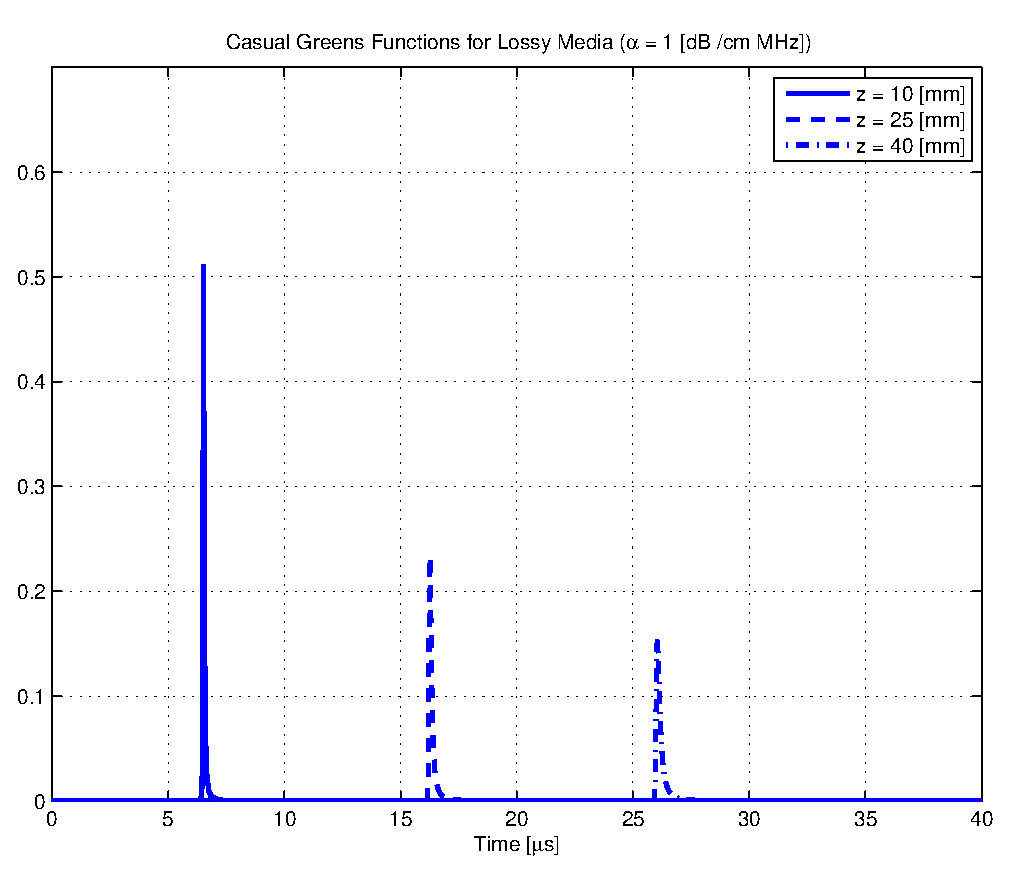
\epsfig{file=userman/eps/lossy_time.eps}}}\quad
    \subfigure[Frequency domain response.
        ]{\scalebox{0.6}{\epsfig{file=userman/eps/lossy_freq.eps}}}
  \end{center}
  \caption{Illustration of the attenuation response at three different depths. The attenuation coefficient, $\alpha$, was
    1 [db/cm MHz] and the attenuation response at 10 mm is the solid line, 25 mm is the dashed line, and 40 mm
    is dash-dotted line, respectively.
    \label{fig:lossy}}
\end{figure}

%\subsection{Far-field approximation}
%
% If the far-field the attanuation resonse are nearly identical so it can be computed outside the DREAM summation
% using a single convolution.
%


\section{A Quick Start to DREAM Simulations}
\label{sec:quick}

\PARstart{I}{n} his section a quick start on how to perform simulations with DREAM is presented. Here only
a simple example is shown just to illustrate what is needed to simulate an ultrasonic measurement system. We
will use a circular transducers for this example but more advanced examples can be found on the DREAM web
page  \url{http://www.signal.uu.se/Toolbox/dream/} on the
\emph{Examples} page. Also more details of the various functions in the DREAM Toolbox can be found in
Sections~\ref{sec:transducer-functions}, \ref{sec:parallel}, and~\ref{sec:misc-functions}, respectively.

Let us study a the pressure response for a circular transducer using water as the propagation
medium (with a sound speed $\cp = 1500$ [m/s]). We start by setting the sampling frequency and defining the
points of interest, the so-called \emph{observation points}. The observation points are located on a line
at $z=10$ mm, from 1--50 mm with 1 mm between them:
\footnotesize
\begin{verbatim}
Fs = 10;   % Sampling freq. in MHz.
Ts = 1/Fs;

%
% Observation point(s).
%

% Depth
z = 10; % [mm]

%  Points along x-axis.
d  = 1;                               % [mm]
xo = (0:d:50);                        % 0-50 mm.
yo = zeros(length(xo),1);
zo = z*ones(length(xo),1);
Ro = [xo(:) yo(:) zo(:)];
\end{verbatim}
\normalsize

Then we need to define the discretization parameters for both the transducer surface and the temporal
sampling:
%
\footnotesize
\begin{verbatim}
% Descretization parameters.
dx = 0.03;                              % [mm].
dy = 0.03;                              % [mm]
dt = Ts;                                % [us].
nt = 400;                               % Length of spatial impulse response vector.
s_par = [dx dy dt nt];
\end{verbatim}
\normalsize

We must also define the sound speed of the medium, normal velocity, and attenuation. Here we choose
an attenuation free medium ($\alpha = 0$) and a unit normal velocity:
\footnotesize
\begin{verbatim}
% Material parameters.
v     = 1.0;                            % Normal velocity.
cp    = 1500;                           % Sound speed.
alpha  = 0;                             % Absorbtion [dB/(cm MHz)].
m_par = [v cp alpha];
\end{verbatim}
\normalsize

The size of the transducer must also be defined, here we use a circular transducer with a
5 mm radius:
\footnotesize
\begin{verbatim}
% Geometrical parameters.
r = 5;                                 % Radius [mm].
geom_par = [r];

\end{verbatim}
\normalsize

Finally we set the start point of the SIR and call the DREAM function \texttt{dreamcirc} to
compute the discrete SIRs:
\footnotesize
\begin{verbatim}
% Delay.
t_z = z*1e3/cp;
%delay = 0;                             % Start at 0 [us].
delay = t_z;                            % Start at t_z [us].

H = dreamcirc(Ro,geom_par,s_par,delay,m_par,'stop');
\end{verbatim}
\normalsize

%
% TODO: add electrical impulse response.
%

\section{Transducer Function Reference}
\label{sec:transducer-functions}

\PARstart{T}{he} transducer functions are implemented as \textsc{Matlab} \emph{mex}-functions
and Octave\ \emph{oct}-functions; a \emph{mex/oct}-function is pre-compiled code that is dynamically
linked to \Matlab/Octave at run time. This greatly increases the computation speed compared to using
ordinary m-files since the DR-concept (see~\cite{Piwakowski1999}) uses \texttt{for} and \texttt{while}
loops extensively. An overview of the transducer functions can be found in Table~\ref{tab:overview}.

% Need a new line above the table otherwise all rows on the table are
% printed on top of each other (bug in latex?).
\begin{table}[tphp]
  \centering
  \begin{tabular}{||l|l||}
    \hline
    \hline
    \textbf{Transducer type} & \textbf{DREAM function} \\
    \hline
    \hline
    Strip transducer & \texttt{dreamline}\\
    Rectangular transducer & \texttt{dreamrect}\\
    Focused rectangular transducer & \texttt{dreamrect\_f}\\
    Circular transducer & \texttt{dreamcirc} \\
    Focused circular transducer & \texttt{dreamcirc\_f}\\
    Spherical concave/convex transducer (defocused/defocused) & \texttt{dreamsphere}\\
    Cylindrical concave/convex transducer (focused/defocused) & \texttt{dreamcylind}\\
    \hline
    Array with rectangular elements & \texttt{dream\_arr\_rect}\\
    Array with circular elements & \texttt{dream\_arr\_circ}\\
    Array with cylindrical concave/convex elements (focused/defocused) & \texttt{dream\_arr\_cylind}\\
    Annular array & \texttt{dream\_arr\_annu}\\
    \hline
    \hline
  \end{tabular}
  \caption{Overview of the DREAM toolbox transducer functions.
    \label{tab:overview}}
\end{table}
%

The transducer functions can be divided in two groups, \emph{single transducer functions} and \emph{array
functions}. The names of both groups starts with ``\texttt{dream}'' and the array functions are distinguished
from single transducer functions by ``\texttt{\_arr\_}''. Note that arbitrary arrays (with mixed forms of
transducer elements) can be modeled using the single transducer functions and then adding their
corresponding responses.

\subsection{Input Parameters Common to all Transducer Functions}


\subsubsection{Observation Point(s) Parameter}
\label{sec:obsarg}

The transducer functions can compute SIRs for multiple observation points. The observation points are given
by a  $N\times 3$ matrix \texttt{Ro} were the first column contains the $x$-coordinates, the second the
$y$-coordinates, and the third the $z$-coordinates, respectively ($N$ is the number of observation points).

The single element transducers are, by convention, all centered at $\mathbf{r} = (0,0,0)$ and the SIRs are
computed relative to this center point.
%
The array functions uses a grid matrix \texttt{G} to define the positions of the array elements
(see Section~\ref{sec:array-par}). The SIRs are therefore computed relative the positions given
by the grid matrix for the arrays.

\subsubsection{Sampling Parameters}
\label{sec:sarg}

The four-element vector \texttt{s\_par = [dx dy dt nt]} determines the spatial discretization and the
temporal sampling properties. The spatial discretization of the transducer surface is given by
\texttt{dx}$\times$\texttt{dy}; small values of \texttt{dx} and \texttt{dy} results in a finer mesh,
and a higher numerical accuracy, compared to larger ones.
%
The temporal sampling interval $\Delta t$ (or $\Ts$) is given by \texttt{dt} and the length of the
SIR-vector is determined by \texttt{nt}. If \texttt{nt} is chosen too low so that any non-zero component
of the SIR is not within the time-window defined by \texttt{[delay dt*(nt-1)+delay]} an error message will
be printed (See Section~\ref{sec:delay} for a description of the \texttt{delay} parameter and
Section~\ref{sec:error} for a description of the error handling in the DREAM toolbox).
%
\begin{description}
\item[\texttt{dx}]  Spatial discretization size in x-direction [mm].
\item[\texttt{dy}]  Spatial discretization size in y-direction [mm].
\item[\texttt{dt}]  Temporal discretization size [$\mu$s] ($\Ts = \Delta t$ = 1/sampling freq).
\item[\texttt{nt}]  Length of spatial impulse response vector.
\end{description}

\subsubsection{The Delay Parameter}
\label{sec:delay}

The starting point of the SIR-vector(s) is given by the delay parameter \texttt{delay} ([$\mu$s]).
The delay parameter can either be a scalar, then all SIRs will have the same starting point, or it can be
a vector with a length that must be equal to the number of observation points. In the latter case each
observation point has a SIR with a different starting point.

%If the delay parameter is set to $|\mathbf{r}_o|/c$ (assuming that the transducer is centered at
%$\mathbf{r} = (0,0,0)$) then the SIR will start at the first index.

\subsubsection{Material Parameters}
\label{sec:material}

The material parameters are given by the three-element vector \texttt{m\_par = [v cp alpha]}:
%
\begin{description}
\item[\texttt{v}]     Normal velocity of the transducer surface[m/s].
\item[\texttt{cp}]    Sound velocity of the medium [m/s].
\item[\texttt{alpha}]  Attenuation coefficient [dB/(cm MHz)]. % (See Appendix~\ref{sec:lossy}).
\end{description}
%
Note: if \texttt{alpha} $\neq 0$ then the SIRs are compensated for attenuation. Note that the attenuation
calculation involves a computation of an inverse discrete Fourier transform of length \texttt{nt} for
every surface element \texttt{dx}$\times$\texttt{dy}~\cite{Piwakowski1999} %(Appendix~\ref{sec:lossy}).
This results in a longer computation time compared to when \texttt{alpha} = 0.
See also Section~\ref{sec:misc-att}.

\subsubsection{Focusing parameters}
\label{sec:focus}


The focusing in the DREAM toolbox is controlled with the two parameters \texttt{foc\_met} and
\texttt{focal}. The \texttt{foc\_met} parameters is a text string that selects the focusing method,
options are:
\begin{description}
\item[\texttt{'off'}]: focusing not used.
\item[\texttt{'x'}]: focus in $x$ only, $\left(\sqrt{x^2 + z_f^2}\right)/\cp$.
\item[\texttt{'y'}]: focus in $y$ only, $\left(\sqrt{y^2 + z_f^2}\right)/\cp$.
\item[\texttt{'xy'}]: focus in both $x$ and $y$, $\left(\sqrt{x^2 + y^2 + z_f^2}\right)/\cp$.
\item[\texttt{'x+y'}]: focus in $x+y$, $\left(\sqrt{x^2 + z_f^2} + \sqrt{y^2 + z_f^2}\right)/\cp$.
\end{description}

%\begin{description}
%\item[\texttt{'off'}]: Focusing not used.
%\item[\texttt{'x'}]: Focus in $x$ only.($t(x,y) = \left(\sqrt{x_\text{max}^2 + z_f^2} -
%  \sqrt{x^2 + z_f^2}\right)/\cp$).
%\item[\texttt{'y'}]: Focus in $y$ only.($t(x,y) = \left(\sqrt{y_\text{max}^2 + z_f^2} -
%  \sqrt{y^2 + z_f^2}\right)/\cp$).
%\item[\texttt{'xy'}] Focus in both $x$ and $y$. ($t(x,y) = \left(\sqrt{x_\text{max}^2 + y_\text{max}^2 + z_f^2}
%  - \sqrt{x^2 + y^2 + z_f^2}\right)/\cp$).
%\item[\texttt{'x+y'}]: Focus in $x+y$. ($t(x,y) = \left(\sqrt{x_\text{max}^2 + y_\text{max}^2 + z_f^2} -
%  (\sqrt{x^2 + z_f^2} + \sqrt{y^2 + z_f^2}\right)/\cp$)).
%\end{description}
%
%where $x_\text{max}$ and $y_\text{max}$ is the size of the transducer in respectively direction, and
%the \texttt{focal} parameter is the focal distance $z_f$ (in [mm]).

This type of focusing is used for the two single transducer functions (\texttt{dreamrect\_f} and
\texttt{dreamcirc\_f} see Section~\ref{sec:single}) and for the array functions (Section~\ref{sec:array}).
The spherical and cylindrical transducer functions also use focusing but there focusing is controlled by
a single parameter \texttt{R} (see Sections~\ref{sec:spher_f}, \ref{sec:spher_d},
\ref{sec:cyl_f}, and \ref{sec:cyl_d}).

\subsubsection{Error Handling}
\label{sec:error}

There are three levels of error reporting for the transducer functions. An error typically occur
when the SIR do not fit within the time window, defined by the delay, sampling period, and
length parameters. The levels are controlled by the optional \texttt{err\_level} parameter which is a text
string with the following alternatives:
%
\begin{enumerate}

\item \texttt{'ignore'}: Here an error is silently ignored,

\item \texttt{'warn'}: An error message is printed but computation is not stopped,

\item \texttt{'stop'}: An error message is printed and the computation is stopped.

\end{enumerate}
%
The error message contains a number that tells how many samples outside the time window the
SIR is. The default error level is \texttt{'stop'} (if the \texttt{err\_level} is omitted).

\subsection{Output Parameters Common to all Transducer Functions}

\subsubsection{The SIR Output Argument}

The first output argument of transducer functions, \texttt{H},  is a matrix or vector,
containing the spatial impulse response(s).
%
\begin{verbatim}
  H = dream***( ... );
\end{verbatim}
%
Each column \texttt{H} contain the SIR for the corresponding entry in the observation point input matrix
\texttt{Ro} (see Section~\ref{sec:obsarg}).

\subsubsection{The Error Output Argument}

The second (optional) output argument, \texttt{err}, is negative if an error has occurred and
0 otherwise.
%
\begin{verbatim}
  [H,err] = dream***( ... );
\end{verbatim}
%
If, for example, \texttt{err\_level = 'ignore'} then no error message will be printed
but \texttt{err} will be negative if an error occurred so the error can be detected. This
is useful for displaying error dialog boxes in GUIs, for example.

%---------------------------------------------------------------

\subsection{Single Element Transducers}
\label{sec:single}

As mentioned above all single element transducers are centered at $\rr = (0,0,0)$. There is, however, no
loss in generality since the response at other transducer positions can simply be obtained
by offsetting the coordinate system after computation.

\subsubsection{Line (strip) Transducer}

The line, or strip, transducer has a length \texttt{a} and a (small) thickness equal to
\texttt{dy} (in \texttt{s\_par}).

\noindent \textbf{Syntax}:
\begin{verbatim}
  H = dreamline(Ro,geom_par,s_par,delay,m_par,err_level);
\end{verbatim}
%
\noindent \textbf{Geometrical parameters}:
\begin{verbatim}
  geom_par = [a];
     a [mm] - length of the strip (in x-direction).
\end{verbatim}

\subsubsection{Rectangular Transducer}

The size of the rectangular transducer is determined by \texttt{a} and \texttt{b}.

\noindent \textbf{Syntax}:
\begin{verbatim}
  H = dreamrect(Ro,geom_par,s_par,delay,m_par,err_level);
\end{verbatim}

\noindent \textbf{Geometrical parameters}:
\begin{verbatim}
  geom_par = [a b];
    a [mm] - x-size.
    b [mm] - y-size.
\end{verbatim}

\subsubsection{Rectangular Focused Transducer}

The size of the rectangular focused transducer is determined by \texttt{a} and \texttt{b} and
the focusing is described in Section~\ref{sec:focus}.

\noindent \textbf{Syntax}:
\begin{verbatim}
  H = dreamrect_f(Ro,geom_par,s_par,delay,m_par,foc_met,focal,err_level);
\end{verbatim}

\noindent \textbf{Geometrical parameters}:
\begin{verbatim}
 geom_par = [a b];
    a [mm] - x-size.
    b [mm] - y-size.
\end{verbatim}

\subsubsection{Circular Transducer}

The size of the circular transducer is determined by the single parameter \texttt{r}.

\noindent \textbf{Syntax}:
\begin{verbatim}
  h  = dreamcirc(Ro,geom_par,s_par,delay,m_par,err_level);
\end{verbatim}

\noindent \textbf{Geometrical parameters}:
\begin{verbatim}
  geom_par = [r];
    r  - Radius of the transducer.
\end{verbatim}

\subsubsection{Focused Circular Transducer}

The size of the focused circular transducer is determined by the parameter \texttt{r}
and the focusing is described in Section~\ref{sec:focus}.

\noindent \textbf{Syntax}:
\begin{verbatim}
  h  = dreamcirc_f(Ro,geom_par,s_par,delay,m_par,foc_met,focal,err_level);
\end{verbatim}

\noindent \textbf{Geometrical parameters}:
\begin{verbatim}
  geom_par = [r];
    r  - Radius of the transducer.
\end{verbatim}

\subsubsection{Spherical Concave Transducer}
\label{sec:spher_f}

\noindent \textbf{Syntax}:
\begin{verbatim}
  H = dreamsphere_f(Ro,geom_par,s_par,delay,m_par,err_level);
\end{verbatim}

\noindent \textbf{Geometrical parameters}:
\begin{verbatim}
 geom_par = [r R];
    r [mm] - Radius of the transducer.
    R [mm] - Curvature radius of the transducer.
\end{verbatim}


\subsubsection{Spherical Convex Transducer}
\label{sec:spher_d}

\noindent \textbf{Syntax}:
\begin{verbatim}
  H = dreamsphere_d(Ro,geom_par,s_par,delay,m_par)
\end{verbatim}

\noindent \textbf{Geometrical parameters}:
\begin{verbatim}
 geom_par = [r R];
    r [mm] - Radius of the transducer.
    R [mm] - Curvature radius of the transducer.
\end{verbatim}

\subsubsection{Cylindrical Concave Transducer}
\label{sec:cyl_f}

\noindent \textbf{Syntax}:
\begin{verbatim}
  H = dreamcylind_f(Ro,geom_par,s_par,delay,m_par,err_level);
\end{verbatim}

\noindent \textbf{Geometrical parameters}:
\begin{verbatim}
 geom_par = [a b R];
    a - x-size of the transducer.
    b - y-size of the transducer.
    R - Radius of the curvature.
\end{verbatim}


\subsubsection{Cylindrical Convex Transducer}
\label{sec:cyl_d}

\noindent \textbf{Syntax}:
\begin{verbatim}
  H = dreamcylind_d(Ro,geom_par,s_par,delay,m_par)
\end{verbatim}

\noindent \textbf{Geometrical parameters}:
\begin{verbatim}
 geom_par = [a b R];
    a - x-size of the transducer.
    b - y-size of the transducer.
    R - Radius of the curvature.
\end{verbatim}

%---------------------------------------------------------------

\subsection{Input Parameters Common to the Array Functions}
\label{sec:array-par}

\subsubsection{The Array Grid Matrix}

The positions of the array transducer elements are determined by the $L\times3$ \emph{grid matrix}
\texttt{G}. The first column contain the (center) $x$-positions of the elements, the second the $y$-positions,
and the third the $z$-positions ($L$ is the number of elements), respectively. This approach is very flexible
and allows for arbitrary array geometries that  not is restricted to equally spaced linear or 2D
arrays.%\footnote{Note that \texttt{G} is a vector for the annular array}.

\subsubsection{Array Focusing}
\label{sec:arrfocus}
%See Section~\ref{sec:focus}.

The array focusing has an extra option, \texttt{'ud'},  compared to the focusing methods described in
Section~\ref{sec:focus}:
\begin{description}
\item[\texttt{'off}]: focusing not used,
\item[\texttt{'x'}]: see Section~\ref{sec:focus},
\item[\texttt{'y'}]: see Section~\ref{sec:focus},
\item[\texttt{'xy'}]: see Section~\ref{sec:focus},
\item[\texttt{'x+y'}]: see Section~\ref{sec:focus}.
\item[\texttt{'ud'}]: user defined focusing.
\end{description}
%
When user defined focusing is used the \texttt{'focal'} parameter is a vector of focusing delays (in $\mu$s).
Each element in \texttt{'focal'} then delays the signal to the corresponding element in the array
(given by the grid matrix).


\subsubsection{Beam Steering Parameters}

The beam steering in the DREAM toolbox is controlled by the two parameters \texttt{steer\_met} and
\texttt{steer\_par}. The \texttt{steer\_met} is a text string with four alternatives:
\texttt{'off'}, \texttt{'x'}, \texttt{'y'}, and \texttt{'xy'}. The \texttt{steer\_par} is a two-element
vector \texttt{steer\_par =  [theta phi]} where \texttt{theta} [deg] is the x-direction steer angle and
\texttt{phi} [deg] the y-direction steer angle.

\subsubsection{Apodization Parameters}
\label{sec:apod}

The DREAM toolbox has five pre-defined apodization windows that can be used
for the array functions:
%
%\begin{equation}
\ifthenelse{\boolean{TEX4HT}}
{
  \begin{eqnarray}
    w_{{triangle}}(r) & = & 1 - \frac{|r|}{r_{{max}}} \\
    w_{{gauss}}(r;p) & = &\exp(-p r^2) / r_{{max}}^2 \\
    w _{{raised}}(r;p) & = & p + \cos(r \pi/r_{{max}}) \\
    w_{{simply}}(r) & = & 1 - r^2 / r_{{max}}^2 \\
    w_{{clamped}}(r) & = & (1 - r^2 / r_{{max}}^2)^2.
  \end{eqnarray}
}{
  \begin{eqnarray}
    w_{\text{triangle}}(r) & = & 1 - \frac{|r|}{r_{\text{max}}} \\
    w_{\text{gauss}}(r;p) & = &\exp(-p r^2) / r_{\text{max}}^2 \\
    w _{\text{raised}}(r;p) & = & p + \cos(r \pi/r_{\text{max}}) \\
    w_{\text{simply}}(r) & = & 1 - r^2 / r_{\text{max}}^2 \\
    w_{\text{clamped}}(r) & = & (1 - r^2 / r_{\text{max}}^2)^2.
  \end{eqnarray}
}
%\end{equation}
%
Additionally to the pre-defined apodizations one can have a user defined apodization weights.
%
Figure~\ref{fig:apod_windows} show some examples of these function.
\begin{figure}[phtb]
  \begin{center}
    \mbox{\subfigure[Triangle]{\scalebox{.3}{\epsfig{file=userman/eps/triangle.eps}}}\hspace{3mm}
      \subfigure[Gaussian]{\scalebox{.3}{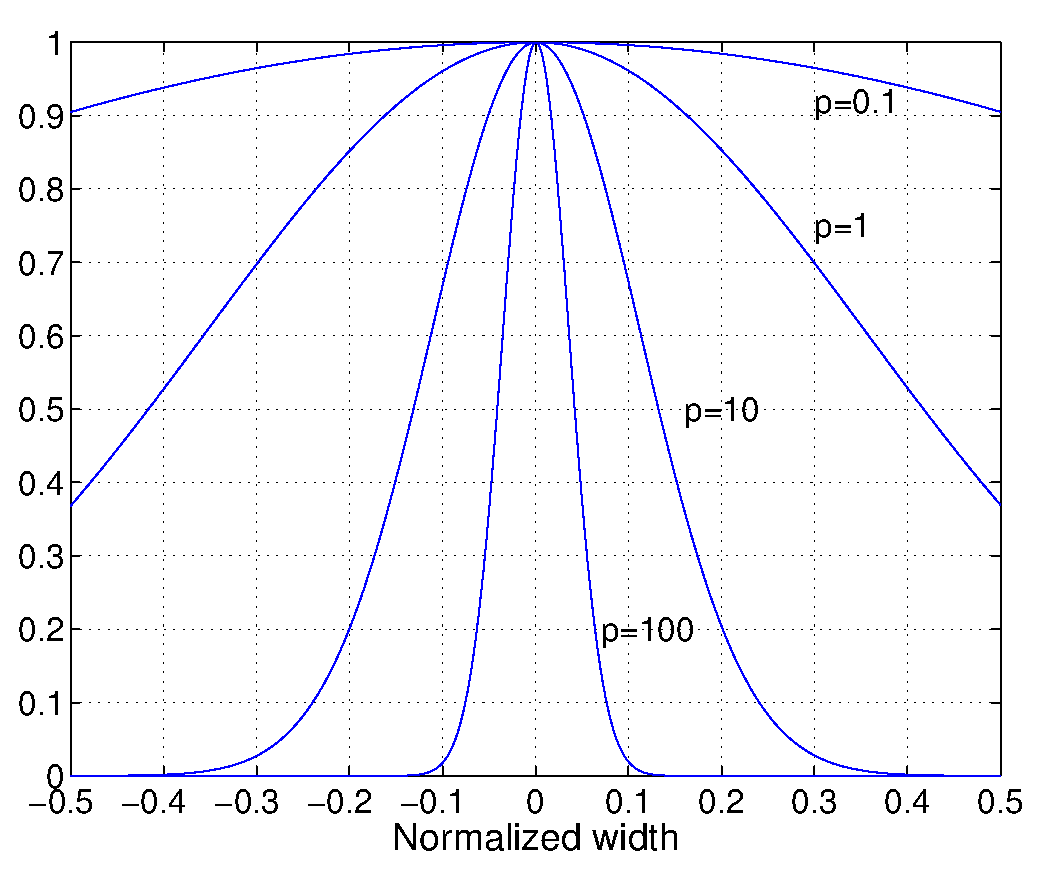
\epsfig{file=userman/eps/gauss.eps}}}\hspace{3mm}
      \subfigure[Raised cosine]{\scalebox{.3}{\epsfig{file=userman/eps/raised.eps}}}}\hspace{3mm}\\
       \mbox{\subfigure[Simply supported]{\scalebox{.3}{\epsfig{file=userman/eps/simply.eps}}}\hspace{3mm}
      \subfigure[Clamped]{\scalebox{.3}{\epsfig{file=userman/eps/simply.eps}}}}
  \end{center}
  \caption{The pre-defined apodization window functions in the DREAM toolbox.
    \label{fig:apod_windows}}
\end{figure}
%

There are three parameters that controls the apodization in the DREAM toolbox, \texttt{apod\_met},
\texttt{apod}, and \texttt{win\_par}.
%
The \texttt{apod\_met} parameter is string variable for selecting apodization method,
options are:
\begin{description}
\item[\texttt{'off'}]      - No apodization
\item[\texttt{'ud'}]       - User defined apodization
\item[\texttt{'triangle'}] - Triangular window
\item[\texttt{'gauss'}]    - Gaussian (bell-shaped) window
\item[\texttt{'raised'}]   - Raised cosine window
\item[\texttt{'simply'}]   - Simply supported
\item[\texttt{'clamped'}]  - Clamped.
\end{description}
%
The second parameter, \texttt{apod}, is a vector of apodization weights that is used for the
\texttt{'ud'} option. Pass an empty matrix (\texttt{[]}) if one of the other options are used.
%
The last parameter, \texttt{win\_par} (scalar), is used for raised cosine and Gaussian apodization
functions. See also Section~\ref{sec:misc-apod}.

\subsection{Array Transducers}
\label{sec:array}

\subsubsection{Array with Rectangular Elements}

\noindent \textbf{Syntax}:
\begin{verbatim}
  H = dream_arr_rect(Ro,geom_par,G,s_par,delay,m_par,foc_met,
        focal,steer_met,steer_par,apod_met,apod,win_par,err_level);
\end{verbatim}

\noindent \textbf{Geometrical parameters}:
\begin{verbatim}
  geom_par = [a b]:
  a  - Element size in x-direction.
  b  - Element size in y-direction.
\end{verbatim}
%\texttt{geom\_par = [a b];}

\subsubsection{Array with Circular Elements}

\noindent \textbf{Syntax}:
\begin{verbatim}
  H = dream_arr_circ(Ro,a,G,s_par,delay,m_par,foc_met,
        focal,steer_met,steer_par,apod_met,apod,win_par,err_level);
\end{verbatim}

Geometrical parameters:
\texttt{r}  - Radius of the transducer elements.


\subsubsection{Array with Cylindrical Concave Elements}

\noindent \textbf{Syntax}:
\begin{verbatim}
  H = dream_arr_cylind_f(Ro,geom_par,G,s_par,delay,m_par,foc_met,
          focal,steer_met,steer_par,apod_met,apod,win_par,err_level);
\end{verbatim}

\noindent \textbf{Geometrical parameters}:
\begin{verbatim}
 geom_par = [a b r]:
   a  - Element size in x-direction.
   b  - Element size in y-direction.
   r  - Radius (y-direction).
\end{verbatim}

\noindent \textbf{Example (linear array)}:
\begin{verbatim}
  gx = -10:1:10;
  gy = zeros(length(gx),1);
  gz = zeros(length(gx),1);
  gx=gx(:);  gy=gy(:);  gz=gz(:);
  G = [gx gy gz];

\end{verbatim}

\subsubsection{Array with Cylindrical Convex Elements}

\noindent \textbf{Syntax}:
\begin{verbatim}
  H = dream_arr_cylind_d(Ro,geom_par,G,s_par,delay,m_par,foc_met,
          focal,steer_met,steer_par,apod_met,apod,win_par,err_level);
\end{verbatim}

\noindent \textbf{Geometrical parameters}:
\begin{verbatim}
 geom_par = [a b r]:
   a  - Element size in x-direction.
   b  - Element size in y-direction.
   r  - Radius (y-direction).
\end{verbatim}

\subsubsection{Annular Array}

\noindent \textbf{Syntax}:
\begin{verbatim}
  H = dream_arr_annu(Ro,G,s_par,delay,m_par,foc_met,focal,apod_met,apod,
          win_par,err_level);
\end{verbatim}

\noindent \textbf{Geometrical parameters}:
\begin{verbatim}
  G  - Vector of annulus radies.
\end{verbatim}
%
The first element in \texttt{G} is the radius of the center element; then \texttt{G}
has two entries for each annulus (the inner and outer radius). Hence, the length of
\texttt{G} must be odd for the annular array.

The \texttt{apod\_met} parameter has the following entries for the annular array function:
\begin{description}
\item[\texttt{'on'}]       - Focusing on (xy), see Section~\ref{sec:focus},
\item[\texttt{'off'}]      - No focusing,
\item[\texttt{'ud'}]       - User defined focusing.
\end{description}


\section{Parallel Processing Support}
\label{sec:parallel}

Since the SIR computation for two different observation points is independent one can easily
divide the observation points in sets and let a different process (or thread) handle each set.
On a multiprocessor machine, where each process (thread) can run on a separate CPU core simultaneously
this will speed up the computations. In the DREAM toolbox this is performed using threads and
the SIRs for each set of observation point set is computed in its own thread.

In DREAM, \href{https://www.cplusplus.com/reference/thread/thread/}{C++11 threads} is used and the number
of CPU cores on the machine is auto-detected to avoid and extra \texttt{n\_cpus} parameter that previously
was used. One can, however, control the number of threads with the \texttt{DREAM\_NUM\_THREADS} environment
variable and on Linux and macOS one can do this using
\footnotesize
\begin{verbatim}
  $ export DREAM_NUM_THREADS=4
\end{verbatim}
\normalsize
%
for example.\footnote{It can also be useful to also adjust the \texttt{OMP\_NUM\_THREADS} and/or
  \texttt{OPENBLAS\_NUM\_THREADS} environment variables which is used on some systems to
  control the number of threads used in the linear algebra backends etc.}

To see if multiple threads are running using Linux or MacOS X, first run a DREAM function on one terminal
%
\begin{verbatim}
    >> H = dreamrect(Ro,geom_par,s_par,delay,m_par,'stop');
\end{verbatim}
%
and, second, open new terminal window and use, for example, the command \texttt{htop}.\footnote{On MacOS X \texttt{htop} can be installed
using Miniconda or MacPorts etc.} One should see something like:
%
\tiny
\begin{verbatim}
  1  [||||||||||||||||||||||||||||||||||||||||||||||||||||||||||||||||||||||||100.0%]     Tasks: 100, 249 thr; 6 running
  2  [||||||||||||||||||||||||||||||||||||||||||||||||||||||||||||||||||||||||100.0%]     Load average: 4.66 2.10 1.04
  3  [||||||||||||||||||||||||||||||||||||||||||||||||||||||||||||||||||||||||100.0%]     Uptime: 4 days, 18:05:06
  4  [||||||||||||||||||||||||||||||||||||||||||||||||||||||||||||||||||||||||100.0%]
  Mem[|||||||||||||||||||||||||||||||||||||||||||||||||||||||||          3052/7925MB]
  Swp[                                                                         0/0MB]

  PID USER      PRI  NI  VIRT   RES   SHR S CPU% MEM%   TIME+  Command
26799 fl         20   0  798M 67020 35492 S 386.  0.8  9:14.40 /usr/libexec/octave/6.2.0/exec/x86_64_pc-linux-gnu/octave-gui
26970 fl         20   0  798M 67020 35492 R 98.6  0.8  0:21.60 /usr/libexec/octave/6.2.0/exec/x86_64_pc-linux-gnu/octave-gui
26969 fl         20   0  798M 67020 35492 R 97.2  0.8  0:21.32 /usr/libexec/octave/6.2.0/exec/x86_64_pc-linux-gnu/octave-gui
26967 fl         20   0  798M 67020 35492 R 96.7  0.8  0:22.08 /usr/libexec/octave/6.2.0/exec/x86_64_pc-linux-gnu/octave-gui
26968 fl         20   0  798M 67020 35492 R 94.8  0.8  0:21.58 /usr/libexec/octave/6.2.0/exec/x86_64_pc-linux-gnu/octave-gui

-snip-
\end{verbatim}
\normalsize
%
As one can see there are four \textsc{Octave} processes running on 100\% on each core instead of just one thread
on one core.

\section{Analytic Transducer  Functions}
\label{sec:analytic}

The DREAM Toolbox has two time-continous analytic functions, and one sampled analytic function, for
circular and a rectangular transducers, respectively~\cite{Stepanishen1971a,Lockwood1973}. The parameters
for the functions,
%
\begin{verbatim}
[Y] = circ_sir(Ro,geom_par,delay,s_par,m_par);

[Y] = rect_sir(Ro,geom_par,delay,s_par,m_par);

[Y] = scirc_sir(Ro,geom_par,delay,s_par,m_par,n_int);
\end{verbatim}
%
are similar to the other DR-based transducer functions, except for the sampled analytic circular function,
\texttt{scirc\_sir}, which has a parameter \texttt{n\_int} that determines the number of points to use
in the (numerical) temporal integration for each sampling interval [cf. Eq.~\eqref{eq:sampled_sir}].

\section{Misc Functions}
\label{sec:misc-functions}

\subsection{Apodization Windows}
\label{sec:misc-apod}

The DREAM toolbox includes function,
%
\begin{verbatim}
   [w] = dream_apodwin(apod_met,a,win_par)
\end{verbatim}
%
that can be used to compute apodization weights using the
methods described is Section~\ref{sec:apod}. The input parameters are:
%
\begin{description}
\item[\texttt{apod\_met}] - Text string for selecting apodization method.
  options are: \texttt{'off'}, \texttt{'ud'}, \texttt{'triangle'}, \texttt{'gauss'},
  \texttt{'raised'}, \texttt{'simply'}, and \texttt{'clamped'}.

\item[\texttt{a}]  - Is the number of points of the apodization window.% (or vector
  %of apodization weights for the \texttt{'ud'} option).

\item[\texttt{win\_par}] - Scalar parameter for raised cosine and Gaussian apodization functions.
\end{description}

\subsection{Attenuation Response}
\label{sec:misc-att}

The function,
\begin{verbatim}
   [H] = dream_att(Ro,s_par,delay,m_par);
\end{verbatim}
%
can be used to compute only the impulse response(s) that is due to attenuation.
The input parameters for \texttt{dream\_att} are:
%
\begin{description}

\item[\texttt{Ro}] - See Section~\ref{sec:obsarg}.

\item[\texttt{s\_par =  [dt,nt];}] - See Section~\ref{sec:sarg}.

\item[\texttt{delay}]  - See Section~\ref{sec:delay}.

\item[\texttt{m\_par= [cp,alpha];}]  -  See Section~\ref{sec:material}.

\end{description}

\subsection{One Dimensional Matrix Convolution Functions}
\label{sec:misc-conv}

The \texttt{conv\_p}, \texttt{fftconv\_p}, and \texttt{fftconv\_ola} functions
computes the one dimensional convolution of the columns in a matrix \texttt{A} and
matrix (or vector) \texttt{B} using one or more threads. These functions
are typically used to compute single-path or double-path (pulse-echo)
responses for a large number of observation points and thus avoiding
a slow \texttt{for}-loop using the build-in \texttt{conv} function
(that only takes vector arguments).

\noindent \textbf{Syntax}:
\begin{verbatim}
  [Y] = conv_p(A,B);
        conv_p(A,B,Y);
        conv_p(A,B,Y,mode_string);
\end{verbatim}

\begin{verbatim}
  [Y] = fftconv_p(A, B)
  [Y, wisdom_string] = fftconv_p(A, B);
  [Y] = fftconv_p(A, B, wisdom_string);
        fftconv_p(A, B, Y, wisdom_string);
        fftconv_p(A, B, Y, mode_string);
        fftconv_p(A, B, Y, mode_string, wisdom_string);
\end{verbatim}

\begin{verbatim}
  [Y] = fftconv_ola(A, B, block_len)
  [Y, wisdom_string] = fftconv_ola(A, B, block_len);
  [Y] = fftconv_ola(A, B, block_len, wisdom_string);
        fftconv_ola(A, B, block_len, Y, wisdom_string);
        fftconv_ola(A, B, block_len, Y, mode_string);
        fftconv_ola(A, B, block_len, Y, mode_string, wisdom_string);
\end{verbatim}

%
where \texttt{A} is an $M\times N$ matrix, \texttt{B} is a $K\times N$
matrix or a $K$-length vector, and \texttt{Y} is the $(M+K-1)\times N$
output matrix.  If $\texttt{B}$ is a vector then each
column in \texttt{A} is convolved with \texttt{B}.

The \texttt{fftconv\_p} performs the convolutions in the frequency
domain using the FFTW library~\cite{fftw} which is significantly
faster than the time-domain implementation \texttt{conv\_p} for long
vectors.\footnote{We have appended a \texttt{\_p} to the function names
  to distinguish them from the non-threaded build-in \texttt{conv} and \texttt{fftconv}
  (availbale in Octave) functions.}

\subsubsection{Using Pre-computed FFTW Plans}

To speed up computation of repeated \texttt{fftconv\_p} operations (of the same size) one can use pre-computed FFTW plans.
First compute the plan for the corresponding vector length,
%
\begin{verbatim}
  [tmp,wisdom_string] = fftconv_p(A(:,1),B(:,1));
\end{verbatim}
%
then use the plan in consecutive computations of the same size,
%
\begin{verbatim}
  for n=1:N

    % Compute new A and B here.

    [Y] = fftconv_p(A,B,wisdom_string);

  end
\end{verbatim}
%
The time-consuming call to FFTW plan functions is then avoided at each call to \texttt{fftconv\_p} inside the loop.

\subsubsection{Using the In-place Mode}

If the involved matrices are large then memory allocation can be time consuming. To alleviate this problem
both \texttt{conv\_p},  \texttt{fftconv\_p} and  \texttt{sum\_fftconv} (see Section~\ref{sec:sumfftconv}) have an in-place
mode that uses a pre-allocated output matrix, hence memory allocation for the (large) output matrix \texttt{Y} is avoided.
For the \texttt{conv\_p} and \texttt{fftconv\_p} functions, the in-place operation has three modes,
\texttt{'='}, \texttt{'+='}, and \texttt{'-='}, respectively.

The default \texttt{'='} mode

\begin{verbatim}

  [Y] = fftconv_p(H,u);

  for n=2:N

    % Compute new H and u here.

    fftconv_p(H,u,Y,'+=');

  end
\end{verbatim}

Note the in-place mode have the side effect that, in the code
%
\begin{verbatim}
    X = Y;
    fftconv_p(H,u,Y,'+=');
\end{verbatim}
%
both \texttt{X} and \texttt{Y} will be altered, since Malab/Octave do not make
a copy of a matrix unless it is changed after the \texttt{X = Y} assignment.

\subsubsection{Computing Array Responses for Arbitrary Input Signals}
\label{sec:sumfftconv}

The pressure response at an observation point $\rr$ can be computed by super-imposing the
responses from the individual array elements. Assume that we have an array with $K$ transmit
elements. The pressure response $p(\rr,t)$ is then given by,
\ifthenelse{\boolean{TEX4HT}}
{
  %%
  \begin{equation}
    p(\rr,t) = \sum_{k=0}^{K-1} h^{{f-}\smt{sir}}_k(\rr,t) * h_{k}^{{ef}}(t) * u_k(t),
    \label{eq:system_impulse_response}
  \end{equation}
  %%
  where $h^{{f-}\smt{sir}}_k(\rr,t)$ is the forward SIR for the $k$th transmit element,
  $h_{k}^{{ef}}(t)$ is the forward electro-acoustical impulse response, and $u_k(t)$ is
  the $k$th input signal.
}{
  %%
  \begin{equation}
    p(\rr,t) = \sum_{k=0}^{K-1} h^{\text{f-}\smt{sir}}_k(\rr,t) * h_{k}^{\text{ef}}(t) * u_k(t),
    \label{eq:system_impulse_response}
  \end{equation}
  %%
  where $h^{\text{f-}\smt{sir}}_k(\rr,t)$ is the forward SIR for the $k$th transmit element,
  $h_{k}^{\text{ef}}(t)$ is the forward electro-acoustical impulse response, and $u_k(t)$ is
  the $k$th input signal.
}
%
The DREAM Toolbox has a function, \texttt{sum\_fftconv}, to facilitate computation of
discrete array responses with arbitrary input signals. Similar to the \texttt{fftconv} function,
the \texttt{sum\_fftconv} function uses a FFT based algorithm to compute the convolutions.
The \texttt{sum\_fftconv} function performs an operation similar to the code:
%%
\begin{verbatim}
  fft_len = M+K-1;
  YF = zeros(fft_len,N);
  for l=1:L
    for n=1:N
      YF(:,n) = YF(:,n) + fft(H(:,n,l), fft_len).* fft(U(:,l), fft_len);
    end
  end
  Y = real(ifft(Y))/fft_len;
\end{verbatim}
%%
where \texttt{H} is a 3D matrix.

\begin{verbatim}
  [Y] = sum_fftconv(U,B);
  [Y] = sum_fftconv(H,U,wisdom_str);
        sum_fftconv(H,U,Y);
        sum_fftconv(H,U,Y,wisdom_str);
\end{verbatim}
%
\noindent Input parameters:
\begin{itemize}

\item [] \texttt{H} An $M\times N\times L$ three-dimensional matrix.

\item [] \texttt{U} A $K\times L$ matrix.

\item [] \texttt{wisdom\_str} Optional parameter (see Section~\ref{sec:misc-conv}).

\end{itemize}
%
and the output parameter, \texttt{Y} , is an $(M+K-1)\times N$ matrix.
%
A typical usage is:
%
\begin{verbatim}

% Compute a new fftw wisdom string.
[tmp,wisdom_str]  = fftconv_p(H(:,1,1),U(:,1));

for i=1:N

  % Do some stuff here.

  Y = sum_fftconv(H,U,wisdom_str);
end
\end{verbatim}
%%
where the overhead of calling FFTW plan functions is now avoided inside the for loop.

\subsection{Parallel Matrix Copy}

The impulse response matrices can often become rather large and the time taken to copy data between matrices
can therefore be considerable. The DREAM Toolbox comes with a threaded function \texttt{copy\_p} to speed up
data copy.

In-place, threaded copy of data into a matrix:
\begin{verbatim}
  copy_p(B,row_idx,col_idx,A);
\end{verbatim}

\noindent Input parameters:
\begin{verbatim}
 B                 - Pre-allocated Output matrix of size >= (r2-r1)x(c2-c1).
 row_idx = [r1 r2] - Two element vector defining rows in B where
                     the data is copied.
 col_idx = [c1 c2] - Two element vector defining columns in B where
                     the data is copied.
 B                 - Input matrix of size (r2-r1)x(c2-c1);
 n_cpus            - Number of threads to use, n_cpus must be greater or equal to 1.
\end{verbatim}

\subsection{The Speed of Sound in Water}

The SIRs are a function of the sound speed in the propagation medium which often is water.
The DREAM toolbox comes with a function \texttt{h2o\_soundspeed}, based on a method by V.A. Del
Grosso~\cite{Grosso1974}, to facilitate computation of the water sound speed (as function
of temperature, pressure, and salinity).

\begin{verbatim}
  [cp] = h2o_soundspeed(T,P,unit,S)
\end{verbatim}

\noindent Input parameters:
\begin{verbatim}
 T    - Temperture [in degrees Celsius].
 P    - Pressure (optional).
 unit - Text string defining the pressure unit of arg 2
        ['Pa','bar','at','atm','mmHg', or, 'psi']  (optional).
 S    - Salinity [in parts per thousand] (optional).
\end{verbatim}


\section{Signal Processing Examples}

% TODO: add intro here.

%\subsection{Harmonic Beampatter Analysis}

\subsection{Double-path Modeling}

Double-path responses can be modeled as convolutions between the forward and backward
responses~\cite{Stepanishen1981}. This operation can be time consuming when the number of
observation points is large. The DREAM toolbox has the threaded functions \texttt{conv\_p}
and \texttt{fftconv\_p} that can be used to speed up this operation.
%
A typical example is:
%
\begin{verbatim}
H = fftconv_p(H_t,H_r); % Double-path.

P = fftconv_p(H,h_e); % Electrical impulse response.
\end{verbatim}
%
where we first compute the double-path SIRs and then add (convolve) the double-path
electrical impulse response to get the (double-path) propagation response matrix \texttt{P}.

\subsection{Synthetic Aperture Imaging --- The Synthetic Aperture Focusing Technique}
\label{sec:saft}

%\PARstart{S}{ynthetic}
Synthetic aperture imaging  (SAI) was developed to improve resolution
in the along track direction for side-looking radar. The idea was to record
data from a sequence of pulses from a single moving real aperture and then, with
suitable computation, combine the signals so the output can be treated as a much
larger aperture. The first synthetic aperture radar (SAR) systems  appeared
in the beginning of the 1950's~\cite{Whiley1985,Sherwin1962}. Later on the method
has carried over to ultrasound imaging in areas such as synthetic aperture sonar
(SAS)~\cite{Gough1997}, medical imaging, and nondestructive
testing~\cite{Seydel1982,Doctor1986}, where the method is often called the synthetic
aperture focusing technique (SAFT).

The conventional time-domain SAFT algorithm performs synthetic focusing
by means of coherent summations, of responses from point scatterers, along
hyperbolas.\footnote{Linear scanning of the transducer is assumed here.}
These hyperbolas simply express the distances, or time-delays, from transducer
positions in the synthetic aperture
to the observation points, see illustration in Figure~\ref{fig:saft}.
%%
\begin{figure}[phtb]
 \begin{center}
   \scalebox{0.6}{\epsfig{file=userman/eps/saft_geometry.eps}}
 \end{center}
\caption{Typical measurement setup for a SAFT experiment. The transducer is mechanically
  scanned along the $x$-axis and at each sampling position, $x_n$,
  $n=0,1,\ldots,L-1$, a data vector (A-scan) of length $K$ is recorded. The
  distance between the transducer, at $(x_n,z=0)$, and the observation point,
  $(x_{\tilde{n}},z_m)$, is given by $R$.
  \label{fig:saft}}
\end{figure}
%%
More specifically, to achieve focus at an observation point $(x_{\tilde{n}},z_m)$, the SAFT
algorithm time shifts and performs a summation of the received signals  $y(x_n,t)$
measured at transducer positions $x_n$  for all $n$ in the synthetic aperture.
The time shifts which aim to compensate for differences in pulse traveling time,
are simply calculated using the Pythagorean theorem and the operation
is commonly expressed in the continuous time
form~\cite{Frazier1998}
%%
\ifthenelse{\boolean{TEX4HT}}
{
  \begin{equation}
    o(x_{\tilde{n}},z_m) = \sum_{n} w_n y(x_n,\frac{2}{\cp}
    \sqrt{(x_{\tilde{n}}-x_n)^2 + z_m^2}).
    \label{eq:saft-c-saft}
  \end{equation}
}{
  \begin{equation}
    o(x_{\tilde{n}},z_m) = \sum_{n} w_n y(x_n,\frac{2}{\cp}
    \sqrt{(x_{\tilde{n}}-x_n)^2 + z_m^2}).
    \label{eq:saft-c-saft}
  \end{equation}
}
%%
where $o(x_{\tilde{n}},z_m)$ is the beamformed image.

The DREAM Toolbox has two functions \texttt{saft} and \texttt{saft\_p}, respectively,
that performs the SAFT operation (with linear interpolation):


% Sampling parameters: s_par = [dt];
%   dt [us] - Temporal discretization period (= 1/sampling freq).
%
% Start point of B-scan data:
%   delay [us] - Scalar delay for all observation points or
%                a vector with individual delays for each
%                observation point.
%
% Material parameters:
% m_par = [cp];
%   cp   [m/s]      - Sound velocity.
%
% Observation point(s) ([mm]):
% Ro = [xo1 yo1 zo2; xo2 yo2 zo2; ... xoN yoN zoN];
%      where N is the number of observation points.
%
% Synthetic aperture:
% a [mm]
%
% Y  - The MxN processed image.
%
% saft is a MEX-function that is a part of the DREAM Toolbox
% available at `http://www.signal.uu.se/Toolbox/dream/'.
%
% Copyright (C

\begin{verbatim}
   Y = saft(B,To,delay,s_par,m_par,Ro,a);
\end{verbatim}

\noindent Input parameters:
\begin{verbatim}
 B     - KxL Ultrasonic B-scan data matrix.
 To    - A matrix of the form  [xo1 yo1 zo2; xo2 yo2 zo2; ... xoL yoL zoL];
         where L is the number of transducer positions.
 delay - A scalar (or vector) of starting point(s) of the A-scans in B.
\end{verbatim}

%A simulation example using the \texttt{saft} function can be found in
%Section~\ref{sec:saft-example}.

\subsection{Delay-and-sum Imaging}
\label{sec:das}

The SAFT method described in Section~\ref{sec:saft} is a special case of methods based on so-called
delay-and-sum imaging (DAS). The simple idea is just to compensate for the double-path propagation delay from
each transmitter/receiver to each observation point and then perform a (coherent) summation. This operation
is essentially based on an geometrical optics approach and is analogous to the operation of an acoustical
lens~\cite{Kino1987}.

The DREAM Toolbox has two functions to facilitate (matrix based) delay-and-sum processing. The two DAS functions
\texttt{das} and \texttt{das\_arr} is similar to the transducer functions in the sense that they return a
matrix with responses corresponding to each observation point. The difference from the transducer functions
is that only the time delay is computed which is represented with a ``1'' at the corresponding index.

The \texttt{das} function is for single transducers and the \texttt{das\_arr} function is for arrays.
The input parameters,
%
\begin{verbatim}
[D,err] = das(Ro,s_par,delay,m_par,err_level)

[D,err] = das_arr(Ro,G,s_par,delay,m_par,foc_met,...
   focal,steer_met,steer_par,apod_met,apod,win_par,err_level)
\end{verbatim}
%
are similar to the ones used in the transducer functions previously described.

% TODO: remove this section?
%\subsection{Model Based Ultrasonic  Array Imaging}

In this section a short introduction to model based ultrasonic imaging is presented. Model based ultrasonic array
imaging~\cite{Stoughton1993,Lingvall2003,Lingvall2007} is different from delay-and-sum imaging in the sense that is
based on optimal information processing  whereas delay-and-sum imaging is based on geometrical focusing. The idea is
to use a (linear) model, taking into account the diffraction effects associated with each transmitter/receiver, the
electrical characteristics for each transmitter/receiver, as well as the used input signal(s), and
then estimate the parameters (the scattering strengths) of the model based on both data and prior
information.
%
The DREAM toolbox can be used in this process for computing the SIRs for the model which can then be convolved
with measured electrical impulse responses to obtain a model for a real measurement setup or using only simulated
impulse responses to evaluate different array designs, for example.

To obtain a linear mode we need to consider both the forward process and the backward process.
As discussed in Section~\ref{sec:analythical} [Eq.~\eqref{eq:pressure_response}] the forward response can be
divided in three parts: the input signal $u(t)$, the forward electro-acoustical response
%
\ifthenelse{\boolean{TEX4HT}}
{
  $h^{ef}(t)$,
}{
  $h^\text{ef}(t)$,
}
and the forward SIR
\ifthenelse{\boolean{TEX4HT}}
{
  $h^{{f-}\smt{sir}}(\r,t)$.
}{
  $h^{\text{f-}\smt{sir}}(\r,t)$.
}
The backward response can similarly be divided in two parts: the
backward acousto-electrical impulse
response
\ifthenelse{\boolean{TEX4HT}}
{
  $h^{eb}(t)$ and the backward SIR $h^{{b-}\smt{sir}}(\r,t)$.
}{
  $h^\text{eb}(t)$ and the backward SIR $h^{\text{b-}\smt{sir}}(\r,t)$.
}
Now, consider an array with $K$ transmit elements and $L$ receive elements and contributions from a single observation
point, $\r = \begin{bmatrix} x &y & z\end{bmatrix}^T$, where ${}^T$ denotes the transpose operator.
The received signal, $y_l(\r,t)$, from the $l$th receive element can be expressed
%%
\ifthenelse{\boolean{TEX4HT}}
{
  \begin{equation}
    \begin{split}
      y_l(\r,t) & =
      \overset{{Forward impulse response (f)}}{\overbrace{\left( \sum_{k=0}^{K-1}
            h^{{f-}\smt{sir}}_k(\r,t) * h_{k}^{ef}(t),
            * u_k(t) \right)}} o(\r) * \\
      & \overset{{Backward impulse response (b)}}{\overbrace{h^{{b-}\smt{sir}}_l(\r,t) *  h_{l}^{eb}(t)}} + e_l(t), \\
      & = h^{f}(\r,t) * h_l^{b}(\r,t) o(\r) + e_l(t), \\
      & = h_l(\r,t) o(\r) + e_l(t),
    \end{split}
    \label{eq:discrete_system_impulse_response}
  \end{equation}
}{
  \begin{equation}
    \begin{split}
      y_l(\r,t) & =
      \overset{\text{Forward impulse response (f)}}{\overbrace{\left( \sum_{k=0}^{K-1}
            h^{\text{f-}\smt{sir}}_k(\r,t) * h_{k}^\text{ef}(t),
            * u_k(t) \right)}} o(\r) * \\
      & \overset{\text{Backward impulse response (b)}}{\overbrace{h^{\text{b-}\smt{sir}}_l(\r,t) *  h_{l}^\text{eb}(t)}} + e_l(t), \\
      & = h^\text{f}(\r,t) * h_l^\text{b}(\r,t) o(\r) + e_l(t), \\
      & = h_l(\r,t) o(\r) + e_l(t),
    \end{split}
    \label{eq:discrete_system_impulse_response}
  \end{equation}
}
%%
where $*$ denotes temporal convolution and $e_l(t)$ is the noise for the $l$th receive element.
Note that the total forward impulse response is a superposition of the forward impulse responses
corresponding to all transmit elements. The \emph{object function}
$o(\r)$ is the scattering strength at the observation point $\r$,
\ifthenelse{\boolean{TEX4HT}}
{
  $h_{k}^{ef}(t)$
}{
  $h_{k}^\text{ef}(t)$
}
is the forward electrical impulse response for the $k$th transmit element,
\ifthenelse{\boolean{TEX4HT}}
{
  $h_{l}^{eb}(t)$
}{
  $h_{l}^\text{eb}(t)$
}
the backward electrical impulse response
for the $l$th receive element, and $u_k(t)$ is the input signal for the $k$th transmit element.
%Hereafter we will refer to the pulse-echo (double-path) impulse $h_l(\r,t)$ as the \emph{system}
%impulse response.

A discrete-time version of~\eqref{eq:system_impulse_response} is obtained by sampling the
impulse responses and by using discrete-time convolutions. If we consider $N$ observation points
then the received discrete waveform from a target at the $n$th observation point,
$\r_n = (x_n,y_n,z_n)$, can be expressed as
%%
\begin{equation}
  \y_l^{(n)} = \h_l^{(n)}(\o)_{n} + \e_l,
  \label{eq:one-pt}
\end{equation}
%%
where the column vector $\h_l^{(n)}$ is the discrete system impulse response for
the $l$th receive element.\footnote{Here all vectors are by convention column vectors.} The vector $\o$
represents the $N$ scattering amplitudes in the region-of-interest, and the notation $(\n)_{n}$ denotes the $n$th
element in $\o$.\footnote{The vector $\o$ can easily be rearrange to form an image when two-dimensional imaging is
  considered~\cite{Lingvall2004}.}
%%

To obtain the received signal for all observation points we need to perform a summation over $n$, which
equivalently can be expressed as a matrix-vector multiplication, according to
%%
\begin{equation}
  \begin{split}
  \y_l = & \sum_{n}\h_l^{(n)}(\o)_{n} + \e_l,\\
  = &\begin{bmatrix} \h_l^{(0)} &  \h_l^{(1)} & \cdots & \h_l^{(N-1)} \end{bmatrix}\o + \e_l,\\
  = & \P_l\o + \e_l,\\
  \end{split}
  \label{eq:all-pts}
\end{equation}
%%
which gives us a liner model for the data for one receive element.

To obtain a model for all elements we can append all $L$ receive signals $\y_l$ into a single vector $\y$ and
we finally have linear model for the total array setup
%%
\begin{equation}
  \begin{split}
    \y = & \begin{bmatrix} \y_{0} \\
      \y_1 \\  \vdots \\
      \y_{L-1}\\  \end{bmatrix}  = \begin{bmatrix} \P_{0} \\
      \P_1 \\  \vdots \\
      \P_{L-1}\\  \end{bmatrix}
    \o +
    \begin{bmatrix} \e_0 \\ \e_1 \\  \vdots \\ \e_{L-1} \\ \end{bmatrix} \\
    = & \P \o + \e,
  \end{split}
  \label{eq:extended}
\end{equation}
%%
for the total array imaging system~\cite{Lingvall2004}.
%
The \emph{propagation matrix}, $\P$, in~\eqref{eq:extended} now
describes both the transmission and the reception process for an arbitrary focused
array. Note that the position of the observation points, and the corresponding scattering amplitudes represented
by the vector $\o$, is not restricted to a regular two-dimensional grid, which is often used in ultrasonic imaging.
%
Furthermore, the array elements can in fact, similar to the observation points , be positioned at arbitrary locations in
tree-dimensional space space. Thus, the model~\eqref{eq:extended} can also
be used to model two-dimensional arrays as well as to model array responses in tree-dimensional space.
Also note that the ``noise'' vector $\e$ describes the \emph{uncertainty} of the model~\eqref{eq:extended}. The noise $\e$
does not only model the measurement noise but also all other errors that we may have, such as: multiple scattering effects,
cross talk between array elements, non-uniform sound speed in the media, etc.

%The DREAM toolbox has a function \texttt{build\_propagation\_matrix} to facilitate computing the propagation
%matrix for a linear array. The function uses a concave linear array transducer function but is should not
%be too difficult for a user to adapt it to other transducer geometries as well.
%After computing the propagation matrix the array system can be simulated by using Eq.~\eqref{eq:extended}.

\subsubsection{The Matched Filter}

The matched filter has the property of maximizing the signal-to-noise ratio (at a single point). The matched filter
for each observation point is given by~\cite{Lingvall2003}
%
\begin{equation}
  \hat{\o}= \P^T\y.
  \label{eq:matched-filter}
\end{equation}

Note that the structure of the matched filter is similar to delay-and-sum processing which  also can be expressed
as a matrix-vector multiplication (see the \texttt{model\_based\_example.m} on the DREAM website),
\begin{equation}
  \hat{\o}= \D^T\y
  \label{eq:das}
\end{equation}
%
where the delay matrix $\D$ has ones in the positions corresponding the the propagation delays and zeros otherwise.

\subsubsection{The Optimal Linear  Estimator}

The optimal linear estimator (or the Wiener filter) is given by~\cite{Stoughton1993,Lingvall2007}
%
\begin{equation}
  \begin{split}
    \hat{\o} & = \Co\P^T(\P\Co\P^T+\Ce)^{-1}\y\\
    & = (\P^T\Ceinv\P+\Coinv)^{-1}\P^T\Ceinv\y,
  \end{split}
\label{eq:optimal}
\end{equation}
%
where $\Co$ is the covariance matrix for $\o$ and $\Ce$ is the covariance matrix for $\e$, respectively.
The estimator~\eqref{eq:optimal} has the property, not found for the matched filter or for delay-and-sum
methods, namely that any beampattern can be compensated given that the signal-to-noise ratio is sufficient.

As a final not on model based imaging is that the matrices involved normally become rather large. It is
therefore highly recommended to used a tuned linear algebra library, such as
\href{http://www.tacc.utexas.edu/resources/software/}{K. Goto's} BLAS library or
the \href{http://math-atlas.sourceforge.net/}{ATLAS} library, for example. These libraries often have thread
support so that all CPUs on the computer can be utilized.

An example of model based (and matrix based delay-and-sum) imaging can be found on the DREAM website (see the
\texttt{model\_base\_example.m} file on the examples page).


\section{The Graphical User Interface (Matlab only)}
\label{sec:gui}

To launch the DREAM Toolbox GUI, type \texttt{dream\_gui} in the \Matlab\ Command
Window %\footnote{The DREAM GUI is not available for Octave.}
and a graphical user interface will be raised as shown in Figure~\ref{fig:gui}.
%
\begin{figure}[phtb]
 \begin{center}
     %\mbox{\scalebox{0.3}{\fbox{\epsfig{file=userman/eps/gui.ps}}}}
     \mbox{\scalebox{0.3}{\fbox{\epsfig{file=userman/eps/gui.eps}}}}
 \end{center}
\caption{The graphical user interface.
\label{fig:gui}}
\end{figure}
%
After activating the user interface, users can set parameters,
compute SIRs, and save and process the resulting SIR by using the
graphical controls. For setting of geometry parameters, please also refer to the
schematic diagram of transducer displayed in the center of the graphic interface.
After setting all the parameters, clicking on the \emph{Compute} button
starts to compute SIR. In addition, the DREAM GUI provides several post-processing
operations to process the SIRs, including computing pressure response, computing the
spectrum of the SIR, and convolving the SIR with an excitation signal. Notice that if
users tick the checkbox of pressure response, the spectrum and
convolution operations will be performed on the pressure instead of on the SIR.
The parameters and resulting SIR can be stored in an \texttt{*.mat} file by clicking on the
button of \emph{Save}.  The parameters settings can then be restored by loading the file using
the \emph{Load} button.
%, or read the
%parameters and process SIR data in the \Matlab\ command window.

% TODO
% \section{Known Issues}

% \begin{itemize}

% \item On Linux, if one get the error\\
%   \texttt{Invalid MEX-file ... libstdc++.so.6: version `GLIBCXX\_3.4.17' not found}\\
%   or similar, then try to pre-load the \texttt{libstdc++.so.6} for the compiler used to build the mex-files. For example,\\
%   \texttt{\$ export LD\_PRELOAD="/usr/lib64/gcc/x86\_64-pc-linux-gnu/4.9.2/libstdc++.so.6"}\\
%   and then start Matlab from the same terminal.

% \item On Windows platforms the MEX-files can not be aborted by
%   pressing \texttt{CTRL-C} since Windows lacks real asynchronous signals, see:
%   %
%   % \begin{verbatim}
%   \url{http://www.mathworks.com/support/solutions/data/1-188VX.html}
%   % \end{verbatim}
%   %
%   Therefore, when \texttt{CTRL-C} is pressed, using Windows, the
%   operation is interrupted after the MEX-file has finished.

% \item On Linux x86 platforms the \Matlab\ release 14 library
%   \texttt{matlab/sys/os/glnx86/libgcc\_s.so} seems to be buggy causing
%   \matlab\ to abort when a \texttt{mexErrMsg} call is done within a
%   MEX-file. The threaded functions uses the \texttt{mexErrMsg}
%   function when \texttt{CTRL-C} is pressed. A work-around is to set the environment
%   variable \texttt{LD\_PRELOAD} to point to a working library. If you, for example, are using
%   gcc 3.4.4, then you can set
%   %
% \begin{verbatim}
%    export LD_PRELOAD=/usr/lib/gcc/i686-pc-linux-gnu/3.4.4/libgcc_s.so
% \end{verbatim}
%   %
%   or rename \texttt{matlab/sys/os/glnx86/libgcc\_s.so} and copy (or
%   link) a working \texttt{libgcc\_s.so} to the
%   \texttt{matlab/sys/os/glnx86/} directory.

% \item The file \texttt{mex\_sum\_fftconv\_p.c} do not compile unless \Matlab\ $\ge$ R2006b is installed. The problem
%   is that \texttt{mwSize} must be defined in \texttt{matlab/extern/include/matrix.h} (\texttt{sum\_fftconv\_p}
%   compiles for Octave).

% \item The computation of responses for lossy media is rather time consuming; the computation time can be as
%   large as a factor of 1000 times longer than for loss-less media. This due to the fact that the frequency
%   domain attenuation response is computed, and an inverse FFT is performed, for every surface element,
%   \texttt{dx}$\times$\texttt{dy}, of the transducer surface.

% \end{itemize}

\newpage

\addcontentsline{toc}{section}{Bibliography}
%\addtocontents{toc}{\protect\contentsline{section}{Bibliography}{\thepage}}

%\bibliographystyle{jasanum.bst}
\bibliographystyle{unsrt}

% Natbib styles
%\bibliographystyle{plainnat.bst}
%\bibliographystyle{abbrvnat.bst}
%\bibliographystyle{unsrtnat.bst}

\bibliography{userman/dream_userman}

\end{document}
